\chapter{Making predictions using PDFs with theoretical uncertainties}
\label{chapter:correlations}
Earlier in this thesis we have discussed the importance of theoretical uncertainties, and how to include them in PDFs. We have also produced PDFs including MHOUs (see Chapter~\ref{chapter:mhous}) and deuteron and nuclear uncertainties (see Chapter~\ref{chapter:nuclear}), which are freely available. In the future, PDFs with theory uncertainties will become the norm, and will be used widely to make theoretical predictions for observables by convoluting them with parton-level hard cross sections. 

When making predictions for hadronic observables there are two sources of uncertainty: the hard cross section and the PDF. Typically, MHOUs for the former are estimated using scale variation, and these are added in quadrature to the latter. When the PDFs themselves also include MHOUs, we can think of the two scale evolutions considered being $Q_0 \to Q_{dat}$ and $Q_0 \to Q_{pred}$, where $Q_0$ is the PDF parametrisation scale, $Q_{dat}$ is the scale of data in the PDF and $Q_{pred}$ is the scale the prediction is made at. Then each of these sources has both a contribution from renormalisation scale variation and from factorisation scale variation.  The PDFs themselves contain data from various processes, so when making a prediction for a process which is included in the PDFs there will invariably be correlations between the renormalisation scale variation in the PDF and that in the hard cross section. Even if the process is a new one, for example Higgs production, correlations due to factorisation scale variation will always be present. Simply combining the two sources of uncertainty in quadrature will miss these correlations and lead to an inflation in overall uncertainties. Hence we refer to this method of combining uncertainties in quadrature as the ``conservative prescription".

This issue was explored in detail in \cite{Harland-Lang:2018bxd}, noting that PDFs are a tool to express one observable in terms of others. This can be realised exactly in the simple case of fully correlated factorisation scale variation for non-singlet structure functions. Here the PDF can be eliminated entirely, and it is manifest that there is only one independent scale ($Q_{dat} \to Q_{pred}$), rather than two, with the MHOUs cancelling to a large degree. If MHOUs were used in both the PDF and the hard cross section in this case, it would amount to ``double counting". It was also shown that correlations existed for renormalisation scale variation, albeit less strongly.

When using PDFs in predictions we include both sources of scale variation in an uncorrelated way, and so miss the MHOU cancellation and corresponding reduction in uncertainties. As noted in \cite{AbdulKhalek:2019ihb}, this is a consequence of PDFs being universal. We cannot reconstruct the full data and MHOUs from the PDFs alone as information is lost in the fitting process; one set of PDFs could arise from many different data possibilities. However, if we want PDFs to be useful in a wide range of predictions, universality is required and so it would at first sight seem like we must live with this loss of correlation.

In \cite{AbdulKhalek:2019ihb} it was argued that we know the increase in PDF uncertainties due to MHOUs is small, and the effect is mostly realised in changes to the central value as the fit is rebalanced by changes to the weighting of different data. Indicative cases were explored in Chapter 7 of the study, where it was seen that the PDF uncertainty is consequently much smaller than the MHOU on the hard cross section. When combining these two in quadrature, the effect of missing correlations was therefore argued to be likely small, and so the overestimate of uncertainty would also be small. It was argued that a small overestimate of uncertainty is better than neglecting MHOUs altogether. It is therefore one of the aims of this study to see whether these claims are justified.

In this chapter we investigate correlations between PDF MHOUs and hard cross section MHOUs when making predictions. Although we focus on MHOUs, the analysis extends naturally to all sources of theory uncertainty. We develop a method for algebraically determining these correlations, and show how to include them when making a prediction. This is a complicated problem so we proceed incrementally:

\begin{itemize}
\item In Sec.~\ref{sec:p1} we show how a theoretical uncertainty can be reformulated in terms of a nuisance parameter, which holds the key to the propagation of uncertainties. We consider two extremal toy models: one where the theory is rigid with no unknown parameters (``pure theory"); the other where the theory is completely flexible and can fit the data exactly (``pure phenomenology"). 
\item In Sec.~\ref{sec:p2} we move on to a model where the data are fitted using just one parameter. Here the correlations lead to a shift in the theoretical predictions. This is somewhere between the two scenarios in Sec.~\ref{sec:p1}.
\item In Sec.~\ref{sec:p3} we extend this analysis to a multi-parameter fit with multiple theory uncertainties, and then to a PDF fit, where the PDFs are continuous functions with a functional uncertainty. 
\item In Sec.~\ref{sec:p4} we present numerical results comparing this procedure with the naive approach of adding the uncorrelated contributions in quadrature, in the context of the NLO global fit with MHOUs discussed in Chapter \ref{chapter:mhous}. We make predictions including MHOUs for repetitions of all the experiments already in the fit (so-called ``autopredictions"). We then investigate the scenario of a prediction for a process already in the fit (top production), and for a new process (Higgs production). We show that including these correlations leads to a shift in the central value of the prediction, which is within the uncertainties for the naive approach but takes the NLO predictions closer to the known NNLO result, reducing the $\chi^2$ to experimental data. Furthermore, we find that for the autopredictions and top predictions there is a significant reduction in uncertainties due to the correlations, so the correlated predictions are both more precise and more accurate. For Higgs production, we find that the effect is much weaker, because there are only correlations through the factorisation scale and not through the renormalisation scale. We emphasise the power of these correlations as a way to improve theoretical predictions.
\item In Sec.~\ref{sec:p5} we provide a summary.
\end{itemize}

\section{Predictions with correlated theory uncertainties}
\label{sec:p1}

We saw in Chapter \ref{chapter:thuncs} that to include theory uncertainties in a fit all you need to do is add a theory covariance matrix, $S_{ij}$, to the experimental covariance matrix $C_{ij}$. Recall that $i,j = 1, \dots, N_{dat}$ run over data points. The only assumptions underlying this result are that all uncertainties are Gaussian, and that the theory uncertainties are independent of the experimental data. Since Gaussian experimental uncertainties are already assumed in NNPDF's framework, these assumptions are very reasonable. We can express the result as the conditional probability
\be
\label{eqn:ptd}
P(T|D) \propto \exp \bigg( -\frac{1}{2} (T-D)^T(C+S)^{-1}(T-D) \bigg).
\ee
Recall that both $C$ and $S$ are real and symmetric, that $C$ is positive definite and that $S$ is positive semidefinite and will generally possess many zero eigenvalues. In a fit we determine $T$ from $D$ by maximising $P(T|D)$, which amounts to minimising
\be
\label{eqn:chi2}
\chi^2 =  (T-D)^T(C+S)^{-1}(T-D)
\ee
with respect to the free parameters which characterise the theory prediction.

In this section we start off by considering one single source of fully correlated theory uncertainty, so that
\be 
S = \beta \beta^T,
\ee
where $\beta$ are real and non-zero. 

\subsection{Nuisance parameters}
\label{subsec:nuis}
We can model the theory uncertainty as a fully correlated shift in the theory prediction:
\be 
T \to T + \lambda \beta,
\ee 
where $\lambda$ is a nuisance parameter characterising the scale of the shift. We will now show that this will lead us to Eqn.~\ref{eqn:ptd}. Firstly, assuming Gaussian experimental uncertainties, we can write
\be 
\label{eqn:nuisptd}
P(T|D\lambda) \propto \exp \bigg( -\frac{1}{2} (T + \lambda \beta -D)^T C^{-1}  (T + \lambda \beta -D) \bigg).
\ee
Using Bayes' Theorem, 
\be 
\label{eqn:bayes}
P(T|D\lambda) P(\lambda |D) \propto P(\lambda | TD)P(T|D).
\ee
We want to find $P(T|D)$, so we need an expression for the prior for $\lambda$, $P(\lambda |D) = P(\lambda)$, where we assume that the theory uncertainty is independent of the experimental data. We choose a unit-width Gaussian centred on zero, 
\be 
\label{eqn:lambdaprior}
P(\lambda) \propto \exp \bigg(-\frac{1}{2} \lambda^2 \bigg).
\ee
Marginalising over $\lambda$, Eqn.~\ref{eqn:nuisptd} becomes
\be 
\label{eqn:ptd2}
P(T|D) \propto \int d\lambda \exp \bigg( -\frac{1}{2} \bigg[ (T + \lambda \beta -D)^T C^{-1} (T + \lambda \beta -D) + \lambda^2 \bigg] \bigg).
\ee
We can evaluate the term in $[ \cdot ]$ by remembering $S= \beta \beta^T$, introducing the variable
\be 
\begin{split}
\label{eqn:z}
Z &\equiv (1 + \beta^T C^{-1} \beta)^{-1} \\
&= 1-\beta^T(C+S)^{-1}\beta \\,
\end{split}
\ee
where the second line comes from the observation that
\be 
(1+\beta^T C^{-1} \beta)(1-\beta^T (C+S)^{-1} \beta) = 1.
\ee
Now completing the square:
\be 
\begin{split}
[ \cdot ] &= (T-D)^T C^{-1}(T-D) + (T-D)^T C^{-1} \lambda \beta + \lambda \beta^T C^{-1} (T-D) \\ &\qquad + \lambda \beta^T C^{-1} \lambda \beta + \lambda^2 \\
& = (T-D)^T C^{-1}(T-D) + (T-D)^T C^{-1} \lambda \beta + \lambda \beta^T C^{-1} (T-D) + \lambda^2 Z^{-1} \\
&=  Z^{-1}(\lambda + Z \beta^T C^{-1} (T-D))^2 \\ &\qquad - Z(\beta^T C^{-1} (T-D))^2 + (T-D)^T C^{-1}(T-D) \\
\end{split}
\ee
so
\be
\begin{split}
[\cdot] &= Z^{-1}(\lambda + Z \beta^T C^{-1} (T-D))^2 \\ &\qquad + (T-D)^T (C^{-1} - Z C^{-1} S C^{-1})(T-D).
\end{split}
\ee
Finally, we can use the Sherman-Morrison formula, which states that for an invertible square matrix, $A$, and column vectors $u$, $v$:
\be 
(A + uv^T)^{-1} = A^{-1} - \frac{A^{-1}uv^TA^{-1}}{1+v^TA^{-1}u}.
\label{eq:ShermanMorrison}
\ee
so we have that
\be 
\begin{split}
(C^{-1} - Z C^{-1} S C^{-1}) &= (C^{-1} - Z C^{-1} \beta \beta^T C^{-1}) \\
&= C^{-1} - \frac{C^{-1}\beta \beta^T C^{-1}}{1+\beta^T A^{-1}\beta} \\
&= (C+S)^{-1},
\end{split}
\ee
so overall
\be 
\begin{split}
[ \cdot ] &= Z^{-1}(\lambda + Z \beta^T C^{-1} (T-D))^2 + (T-D)^T (C + S)^{-1}(T-D) \\
&= Z^{-1}(\lambda + Z \beta^T C^{-1} (T-D))^2 + \chi^2 \\
&\equiv Z^{-1}(\lambda - \bar{\lambda}) + \chi^2,
\end{split}
\ee
where we used the definition of the $\chi^2$ (Eqn.~\ref{eqn:chi2}) and we have defined 
\be 
\begin{split}
\label{eqn:lambdabardef}
\bar{\lambda} &= Z \beta^T C^{-1} (D-T) \\
&= \frac{\beta^T C^{-1}}{1+\beta^T C^{-1} \beta} (D-T)\\
&= \frac{\beta^T}{C+\beta \beta^T} (D-T) \\
&= \beta^T (C+S)^{-1}(D-T),
\end{split}
\ee
where to get to the second line we used the definition of $Z$ (Eqn.~\ref{eqn:z}).
Plugging this back into Eqn.~\ref{eqn:ptd2}, we get
\be  
\begin{split}
\label{eq:margresult}
P(T|D) &\propto \int d\lambda \ e^{-\frac{1}{2} \chi^2} \exp \bigg( -\frac{1}{2} Z^{-1} (\lambda - \bar{\lambda})^2 \bigg) \\
&\propto e^{-\frac{1}{2} \chi^2},
\end{split}
\ee
which is Eqn.~\ref{eqn:ptd}. The advantage of this approach is that we can also get the posterior distribution for $\lambda$ (after fitting using $D$ and $T$), by using Bayes' Theorem (Eqn.~\ref{eqn:bayes}):
\be 
\begin{split}
\label{eqn:lambdaposterior}
P(\lambda |TD) &= \frac{P(T|D\lambda) P(\lambda)}{P(T|D)} \\
&\propto \exp \bigg( -\frac{1}{2} \bigg[ (T+ \lambda \beta -D)^T C^{-1}(T+ \lambda \beta -D) + \lambda^2 - \chi^2 \bigg] \bigg) \\
&\propto \exp \bigg( -\frac{1}{2} Z^{-1}(\lambda - \bar{\lambda})\bigg),
\end{split}
\ee
where we recognised the similarity between the exponent here and in Eqn.~\ref{eqn:ptd2}. So the effect of the fit is to shift the centre of the distribution from 0 $\to \bar{\lambda}$, and the width from 1 $\to Z$. Note that from the definition of $Z$ (Eqn.~\ref{eqn:z}), 
\be 
0 \le Z \le 1,
\ee
so the theory uncertainty is always reduced when information on $D$ is added. Fig.~\ref{fig:lambdadistribs} gives a sketch of this effect.  
%%%%%%%%%%%%%%%%%%%%%%%%%%%%%%%%%%%%%%%%%%%%%%%%%%%%%%%%%%%%%%%%%%%%%
\begin{figure}[H]
  \begin{center}
      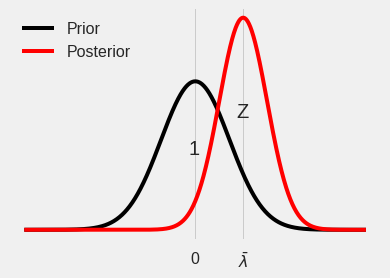
\includegraphics[width=0.5\textwidth]{correlations/plots/lambdapriorpost.png}
    \caption{Sketch of the prior (Eqn.~\ref{eqn:lambdaprior}) and posterior (Eqn.~\ref{eqn:lambdaposterior}) distributions for $\lambda$. Adding information shifts the distribution and reduces the width. \label{fig:lambdadistribs}}
    
  \end{center}
\end{figure}
%%%%%%%%%%%%%%%%%%%%%%%%%%%%%%%%%%%%%%%%%%%%%%%%%%%%%%%%%%%%%%%%%%%%%%

\subsection{Predictions without fits}
We will now test out this formalism for a toy model where we have ``pure theory" values, $T_0$. These have no unknown parameters, so cannot be fitted. They do, however, have a theory uncertainty. Despite the fact we cannot fit them to the data, $T_0 \neq D$ in general, the data can still give us information on the predictions via the nuisance parameters in the theory uncertainties. The expectation value of $\lambda$ can be evaluated 
\be
E[\lambda] = \mathcal{N}_\lambda \int d\lambda \ \lambda\ P(\lambda |T_0 D) = \bar{\lambda}(T_0,D).
\ee
Note that $\mathcal{N}_\lambda$ is set such that $E[1]=1$. We can then find the variance
\be 
\Var[\lambda] \equiv E[(\lambda - E[\lambda])^2] = Z.
\ee
Both of these can be seen straight away from the form of the posterior for $\lambda$, Eqn.~\ref{eqn:lambdaposterior}.

In the nuisance parameter formalism, we can write 
\be 
T(\lambda) = T_0 + \lambda \beta.
\ee
Before comparing these theory predictions to the data, we could use the prior for $\lambda$ in this expression, which would give us
\be 
E[T(\lambda)] = T_0, \qquad \Cov[(T(\lambda)] = \beta \beta^T = S.
\ee
But we could instead first compare $T$ to $D$, and then use the posterior distribution. In that case we'd end up with
\be
\label{eqn:expT}
\begin{split} 
E[T(\lambda)] &= T_0 + \bar{\lambda}(T,D)\beta \\
&= T_0 + \beta \beta^T (C+S)^{-1} (D-T_0) \\
&= T_0 + S(C+S)^{-1} (D-T_0),
\end{split}
\ee
where we substituted Eqn.~\ref{eqn:lambdabardef} to get to the second line,
and
\be 
\begin{split}
\Cov[(T(\lambda)] &= E[(T(\lambda) - E[T(\lambda)])^2] \\
&= \Var[\lambda] \beta \beta^T \\
&= ZS.
\end{split}
\ee 
We can think of these predictions as ``autopredictions", i.e. we:
\begin{enumerate}
\item compare the data to the theory;
\item use the information from 1. to make new predictions for exact repetitions of the same experiments.
\end{enumerate}
From Eqn.~\ref{eqn:expT} we can see that there is a shift in the autopredictions of
\be 
\label{eqn:autoshift1}
\delta T = -S(C+S)^{-1}(T_0-D),
\ee
and that the uncertianties are reduced by a factor $\sqrt{Z}$, thanks to information provided by the data. Overall, the autoprediction covariance matrix is
\be 
\begin{split}
ZS &= S - S(C+S)^{-1}S \\
&= C(C+S)^{-1}S = S(C+S)^{-1}C.
\end{split}
\ee 
To see the impact of the shift in the predictions, we can compare the experimental $\chi^2$ (i.e. using the experimental covariance matrix only) of the original predictions to the autopredictions. The original $\chi^2$ is
\be  
\chi^2_{exp} = (T_0-D)^T C^{-1} (T_0-D),
\ee
and, using Eqn.~\ref{eqn:autoshift1}, the autoprediction $\chi^2$ is
\be
\begin{split} 
\chi^2_{auto} &= (T_0 + \delta T - D)^T C^{-1} (T_0 + \delta T -D) \\
&= (T_0 - S(C+S)^{-1}(T_0-D)-D)^TC^{-1}(T_0 - S(C+S)^{-1}(T_0-D)-D) \\
&= ((1-S(C+S)^{-1})(T_0-D))^TC^{-1}((1-S(C+S)^{-1})(T_0-D)) \\
&= (C(C+S)^{-1}(T_0-D))^TC^{-1}(C(C+S)^{-1}(T_0-D)) \\
&= (T_0-D) (C+S)^{-1} C (C+S)^{-1} (T_0-D),
\end{split}
\ee
where we used Eqn.~\ref{eqn:autoshift1} to get to the second line.
From this we can see that $\chi^2_{auto} \leq \chi^2_{exp}$ because $C+S$ is positive definite. In other words, the shifts always lead to improved quality of fit by exploiting the theory uncertainty to add information from the data.

We can investigate this more explicitly by using a simple model where the experimental covariance matrix is diagonal and the theory uncertainty is fully correlated. Writing $\beta = s e$, where $s$ is the size of correlated theory uncertainty and $e^Te=1$, we have
\be
\label{eq:modelCS}
C = \sigma^2 \mathbb{I},\qquad S = s^2 e e^T,
\ee
where $\sigma$ is the per-point uncertainty. Then we can evaluate:
\be
\begin{split}
\label{eq:modelCplusSinv}
(C+S)^{-1} &= \frac{1}{\sigma^2}\left(1-\frac{s^2}{\sigma^2+s^2}e e^T\right); \\
Z &= (1+s^2/\sigma^2)^{-1}.
\end{split}
\ee
so the reduction in the theory uncertainties depends on $s^2/\sigma^2$:
\begin{itemize}
\item for $s^2 \ll \sigma^2$, there is a small influence of the data on the theory uncertainty;
\item for $\sigma^2 \ll s^2$, the theory uncertainty size is reduced from $s$ to $\sigma$, because in the limit $s^2/\sigma^2 \to \infty$, $Z \to \sigma^2 ee^T$;
\item for theory uncertainties the same size as experimental ones, $\sigma^2 \sim s^2/N$ and $Z \sim 1/(N+1)$, so if there are a large number of independent data points then there is a large reduction in uncertainty; more data gives more information.
\end{itemize}
In this model the autoprediction shifts are
\be 
\delta T = \frac{-s^2}{\sigma^2 + s^2} e^T (T_0-D)e,
\ee
which are in the direction of the theory uncertainty, $e$, as we would expect. When $s^2/\sigma^2 \to \infty$, $e^T(T_0 + \delta T) \to e^T D$, so in this direction the autopredictions coincide with the data.

It can also be shown that the autoprediction $\chi^2$ is
\be 
\chi^2_{auto} = (T_0-D)^T \frac{1}{\sigma} \bigg(1- \frac{s^2(s^2+2\sigma^2)}{(s^2 + \sigma^2)^2} e e^T \bigg) (T_0-D),
\ee 
so the contributions to the $\chi^2$ which are orthogonal to $e$ are unchanged, and the contributions along $e$ are reduced by $Z^2$. This means unless the theory uncertainties are very small, we will end up with a $\chi^2$ for the autopredictions which is size $(N-1)$ rather than $N$, because the contribution along $e$ will be substantially reduced.

We can also make genuine predictions, $\Ttil_I$, $I=1,\dots \ \widetilde{N}$. In this scenario these also have no free parameters, but their theory uncertainty is correlated with that of $T_i$, $i=1, \dots , N$, for which we have experimental data, $D_i$. We can write the predictions in the nuisance parameter formalism as
\be 
\Ttil(\widetilde{\lambda}) = \Ttil + \widetilde{\lambda} \widetilde{\beta},
\ee
where the vector $\widetilde{\beta}$ gives the size and direction of the theory uncertainty in $\Ttil$. If $\widetilde{\lambda}$ are independent of $\lambda$, then the theory uncertainties in $\Ttil$ are uncorrelated with those in $T$ and the covariance for the predictions is just
\be 
\Stil = \betatil \betatil^T.
\ee
In the opposite scenario where they are fully correlated, $\lambdatil = \lambda$ and we can use the data $D$ for $T$ to improve our prediction by using the posterior of $\lambda$, i.e. $P(\lambda|TD)$:
\be 
\begin{split}
E[\Ttil (\lambda)] &= \Ttil + \overline{\lambda} (T,D) \betatil \\
&= \Ttil + \betatil \beta^T (C+S)^{-1} (D-T),
\end{split}
\ee 
where once again we have used Eqn.~\ref{eqn:lambdabardef} to get to the second line.
So there is a shift in the predictions of 
\be 
\label{eq:shiftpred}
\delta \Ttil = - \Shat (C+S)^{-1} (T-D),
\ee
where $\Shat = \betatil \beta^T$ is the covariance matrix of cross correlations between the theory uncertainty in the theory for which there are data and that in the predictions. The covariance matrix of the predictions can be calculated 
\be
\begin{split}
\Cov[\Ttil(\lambda)] &\equiv E[(\Ttil(\lambda) - E[\Ttil(\lambda)]^2) \\
&= E[((\lambdatil - \overline{\lambda})\betatil)((\lambdatil - \overline{\lambda})\betatil)^T]\\
&= \Var[\lambda] \betatil \betatil^T \\
&= Z \Stil.
\end{split}
\ee
So the covariance of the genuine predictions is reduced by the same factor, $Z$, as the autopredictions. This means the data can work via the correlations in theory uncertainties to produce more precise and (if the theory is correct) more accurate predictions for observables that aren't yet measured. This is accompanied by a shift which is proportional to the cross covariance between theory uncertainties.

We can understand a little more about the various theory covariance matrices by imagining we obtained some experimental measurements, $\widetilde{D}$, corresponding to predictions $\Ttil$. Then we could add these to the fit, and would get a new fitting theory covariance matrix with dimensions $(N+\widetilde{N})\times(N+\widetilde{N})$ and content
\be
\left(\begin{array}{cc}
S&\Shat\\
\Shat^T&\Stil\end{array}\right)
 =
\left(\begin{array}{cc}
\beta\beta^T&\beta\betatil^T\\
\betatil\beta^T&\betatil\betatil^T\end{array}\right).
\label{eq:covmatglobal}
\ee
Here the role of $\Shat$ and $\Shat^T$ as cross-correlation theory covariance matrices is clear. We can see that the theory uncertainties in the prediction are consistent with the theory uncertainties we would use when including observables in a fit, which makes sense in the comparison with the autopredictions case. 

Ideally, the shifted predictions would give a better $\chi^2$ to the new data $\widetilde{D}$, but this is not guaranteed because the shifts were induced from the old data, $D$, and there could be inconsistencies between $D$ and $\widetilde{D}$.

\subsection{Autopredictions in a perfect fit}
We have just considered the scenario where $T$ is unfitted to the data. Now consider the ``opposite" situation of a perfect fit. Here $T$ have a high level of flexibility, and can fit $D$ exactly. $P(T|D)$ is always maximised when $T=D$, so $\chi^2=0$. We can extract the expectation value and covariance of $T$ as 
\be 
E[T] = \mathcal{N}_T \int\ dT\ T\ P(T|D) = D,
\ee 
where $\mathcal{N}_T$ is such that $E[1]=1$, and
\be 
\label{eq:varTpheno}
\Cov[T] \equiv E[(T-E[T])^2] = C+S.
\ee
We can write the autopredictions again in the nuisance parameter formalism, so
\be 
T(\lambda) = T + \lambda \beta.
\ee 
When calculating the expectation value of a function of $T$ and $\lambda$, we must take some care. The data, $D$ are always held fixed because they are set values from experiment. Then the expectation value can be calculated using conditional probabilities,
\be 
E[f(T, \lambda)] \equiv \mathcal{N}_T \int dT\ \mathcal{N}_\lambda \int d\lambda\ f(T,\lambda) P(\lambda|TD)P(T|D).
\ee
We must therefore integrate first over $\lambda$, because this is conditional on $T$, and then over $T$. So to get the expectation value of $\lambda$, we first take the expectation value over $\lambda$, with both $T$ and $D$ fixed, using the definition of $\overline{\lambda}$ from Eqn.~\ref{eqn:lambdabardef}:
\be 
\begin{split}
E[\lambda] &= E[\overline{\lambda}(T,D)] \\
&= \beta^T (C+S)^{-1} E[D-T].
\end{split}
\ee
Then we take the expectation value over $T$, keeping $D$ fixed, which just gives us
\be
E[\lambda] = \beta^T (C+S)^{-1} (D-D) =0.
\ee
For the variance we have
\be 
\Var[\lambda] = E[(\lambda-E[\lambda])^2] = E[\lambda^2].
\ee
To evaluate this we can use the trick of adding and subtracting $\overline{\lambda}(T,D)$ to $\lambda$ because we are aiming to put it in terms of $Z = E[(\lambda-\overline{\lambda}(T,D))^2]$. Making use of Eqn.~\ref{eqn:z} and Eqn.~\ref{eq:varTpheno},
\be 
\begin{split}
\Var[\lambda] &= E[(\lambda - \overline{\lambda}(T,D) + \overline{\lambda}(T,D))^2] \\
&= E[(\lambda-\overline{\lambda}(T,D))^2] + E[\overline{\lambda}(T,D)^2] \\
&= Z + \beta^T (C+S)^{-1} E[(T-D)(T-D)^T] (C+S)^{-1} \beta \\
&= Z + \beta^T (C+S)^{-1} \Cov[T] (C+S)^{-1} \beta \\
&= 1 - \beta^T(C+S)^{-1} \beta + \beta^T (C+S)^{-1} \beta \\
&= 1. 
\end{split}
\ee
So in a perfect fit, the posterior distribution of nuisance parameters is exactly the same as the prior. All the information from the data is absorbed into the fitted parameters, and so we are left with no update to the theoretical uncertainty. In the calculation of the variance you can see how the reduction by factor $Z$ that we saw in the pure theory case is exactly cancelled by the factor due to the fluctuation of $\overline{\lambda}(T,D)$ due to the covariance of $T$.

We can now use the posterior of $\lambda$ to calculate the autopredictions. First we calculate the expectation value:
\be 
E[T(\lambda)] = E[T + \lambda \beta] = D,
\ee
which is a consistency check. Next we calculate the covariance, where we remember the expectation value is taken first over $\lambda$ with $T$ and $D$ fixed, and then over $T$ with $D$ fixed: 
\be 
\begin{split}
\label{eqn:covtlam}
\Cov[T(\lambda)] &= E[(T(\lambda)-E[T(\lambda)])^2] \\
&=E[(T-D+\lambda \beta)(T-D+\lambda \beta)^T] \\
&=E[(T-D)(T-D)^T] + E[\lambda \beta (T-D)^T]\\ &\qquad + E[(T-D) \lambda \beta^T] + E[\lambda^2] \beta \beta^T.
\end{split}
\end{equation}
The first term is just $\Cov[T]$ and the last term is $\Var[\lambda] S=S$. To calculate the middle terms, consider
\be
\begin{split}
E[\lambda \beta (T-D)^T] &= E[\beta \overline{\lambda}(T,D)(T-D)^T] \\
&=-S(C+S)^{-1}E[(T-D)(T-D)^T] \\ 
&=-S(C+S)^{-1}\Cov[T].
\end{split}
\ee
So overall
\be 
\begin{split}
\Cov[T(\lambda)] &= \Cov[T] - S(C+S)^{-1}\Cov[T] - \Cov[T](C+S)^{-1}S + \Var[\lambda] S \\
&= (C+S) -S -S +S \\
&=C.
\end{split}
\ee
So in a perfect fit, the covariance of the autopredictions is equal to the covariance of the data. This happened because the covariance arising from the fit (the first term in Eqn.~\ref{eqn:covtlam}), and the covariance arising in the autopredictions (the last term in Eqn.~\ref{eqn:covtlam}) are each cancelled by the cross covariance between the fit and the prediction. This is the effect which was noted in \cite{Harland-Lang:2018bxd}. In a perfect fit, there is no distinction between the autopredictions and the data, and so the theory uncertainty is irrelevant. In other words, the case of a perfect fit can be thought of as ``pure phenomenology"; the only information we are left with is in the data. As a result we can't make genuine predictions for points we don't have experimental data for because there's no real underlying theory.

\section{One-parameter fits}
\label{sec:p2}
Previously, we looked at two unrealistic simple models;
\begin{enumerate}
\item Fixed theory which cannot be fitted to data (pure theory);
\item Over-flexible theory which is fitted perfectly to data (pure phenomenology).
\end{enumerate}
These helped us to develop the nuisance parameter approach, but in reality we want somewhere between these two extremes; normally the theory has parameters which are constrained by the data and can be fitted, however the theory is rigid enough to be able to make new predictions, $\Ttil$, where no data exist. We will see that in this more realistic case there are features from both the pure theory and the pure pheno cases, namely:
\begin{enumerate}
\item shifts in the central values;
\item reduction in uncertainty;
\item correlations of theory uncertainties.
\end{enumerate}
First we will consider a theory with one fitted parameter. Then we will generalise this to many fitted parameters, which is a description of many modern PDF fits. Finally, we will consider an NNPDF fit, where the many parameters are encapsulated in a neural network. 

Starting with the single parameter fit, $T(\theta)$ only depend on a single parameter, $\theta$. The $\chi^2$ (Eqn.~\ref{eqn:chi2}) will be minimised for some $\theta = \theta_0$, with variance $\Var [\theta]$. Once $\theta_0$ has been determined we can then make some predictions, $\Ttil(\theta_0)$, where the tilde denotes they are predictions for theories separate from the fit inputs. These predictions will have uncertainties proportional to $\Var [\theta]$. 

We have assumed that the uncertainties are Gaussian, and so they are differentiable. This means we can linearise $T(\theta)$ about $T(\theta_0) \equiv T_0$:
\be
\label{eq:Tlin}
T(\theta) = T_0 + (\theta-\theta_0)\Tdot_0 + \dots .
\ee
We want to determine the uncertainty in the fitted $\theta$, so we need to propagate the uncertainties in the data, $D$, and the theory, $T(\theta)$, into $\theta$. We can do this using the standard NNPDF approach (see Chapter ~\ref{chapter:background}) of generating pseudodata replicas, $D^{(r)}$, which are Gaussianly distributed about the actual data, $D$, with covariance $C+S$. It is important to remember that these are just a device for propagating the uncertainty, and we must still hold $D$ constant when taking expectation values. More explicitly, we can define the average over replicas for any function, $F$, of the replicas as
\be
\label{eq:repav}
\langle F(D^{(r)})\rangle = \lim_{N_{rep} \to \infty} \smallfrac{1}{N_{\rm rep}}\sum_{r=1}^{N_{\rm rep}}F(D^{(r)}).
\ee
Then the replicas will satisfy
\be 
\label{eq:repavD}
\langle D^{(r)}\rangle \equiv D, \qquad \langle (D^{(r)}-D)(D^{(r)}-D)^T\rangle = C+S.
\ee
in the limit of $N_{rep} \to \infty$.

The fit proceeds by fitting a parameter replica, $\theta^{(r)}$, for each pseudodata replica, $D^{(r)}$, by minimising
\be
\label{eq:chi2rep}
\chi_r^2[\theta] = (T(\theta)-D^{(r)})^T(C+S)^{-1}(T(\theta)-D^{(r)}),
\ee
with respect to $\theta$. Using Eqn.~\ref{eq:Tlin}, this leads to 
 \be
\label{eq:arep}
\theta^{(r)} - \theta_0 = \frac{\Tdot_0^T(C+S)^{-1}(D^{(r)}-T_0)}{\Tdot_0^T(C+S)^{-1}\Tdot_0}.
\ee
Now $\theta_0 = \langle \theta^{(r)} \rangle$, so using the replica averages in Eqn.~\ref{eq:repavD} we find
\be
\label{eq:consistency}
\Tdot_0^T(C+S)^{-1}(D-T_0)=0,
\ee
so we can rewrite Eqn.~\ref{eq:arep} as
\be
\label{eq:arep2}
\theta^{(r)} - \theta_0 = \frac{\Tdot_0^T(C+S)^{-1}(D^{(r)}-D)}{\Tdot_0^T(C+S)^{-1}\Tdot_0}.
\ee
Using the fact that $C$ and $S$ are symmetric, 
\bea
\Var[\theta] &=& \langle(\theta^{(r)}-\theta_0)^2\rangle\nn\\
 &=& \frac{\Tdot_0^T(C+S)^{-1}\langle(D^{(r)}-D)(D^{(r)}-D)^T\rangle (C+S)^{-1}\Tdot_0}{(\Tdot_0^T(C+S)^{-1}\Tdot_0)^2}\nn\\
&=& (\Tdot_0^T(C+S)^{-1}\Tdot_0)^{-1}.
\label{eq:vara}
\eea
Note that:
\begin{itemize}
\item data points with a large dependence on $\theta$ have large $\Tdot_0$ and contribute more.
\item directions with large uncertainty, $(C+S)$, contribute less.
\end{itemize}
Now we have the uncertainty in the fitted parameter, $\theta$, we can find the fitting uncertainty. This is the covariance of $T(\theta)$ due to the experimental and theoretical uncertainties from fitting $\theta$. We will call this covariance matrix $X$. Using the fact that $E[T] = \langle T(\theta^{(r)})\rangle = T(\theta_0) = T_0$ and writing $T^{(r)} = T(\theta^{(r)})$,
\bea
X\equiv\Cov[T(\theta)] &=& \langle(T^{(r)}-T_0)(T^{(r)}-T_0)^T\rangle\label{eq:Xdef}\\
&=& \Tdot_0\langle(\theta^{(r)}-\theta_0)^2\rangle\Tdot_0^T\\
&=& \Tdot_0(\Tdot_0^T(C+S)^{-1}\Tdot_0)^{-1}\Tdot_0^T\label{eq:Xdef2}\\
&=& n(n^T(C+S)^{-1}n)^{-1}n^T,
\label{eq:Xdef3}
\eea
where in the last line we define $\Tdot_0 \equiv |\Tdot_0|n$, i.e. $n$ is a unit vector in the direction of $\Tdot_0$. We can see that $X$ depends only on the direction ($n$) of $\Tdot_0$, not its magnitude. Note that $X$ is singular and also that
\be
\label{eq:XsqeqX}
X = X(C+S)^{-1}X,
\ee
which will be useful later. Using Eqn.~\ref{eq:arep2} in Eqn.~\ref{eq:Tlin}, we can see that
\be
T^{(r)}-T_0 = X(C+S)^{-1}(D^{(r)}-D^{(0)}),
\label{eq:projection}
\ee
so $X(C+S)^{-1}$ projects the data replicas onto the theory replicas.

Now let's revisit the model for covariance matrices, Eqn.~\ref{eq:modelCS}. If we define the angle between the theoretical uncertainties and the $\theta$ variation by $\cos \phi = n^T e$, we find that
\bea
\label{eq:denom}
n^T(C+S)^{-1}n &=& \frac{\sigma^2+s^2\sin^2\phi}{\sigma^2(\sigma^2+s^2)},\\
n^TXn &=& \frac{\sigma^2(\sigma^2+s^2)}{(\sigma^2+s^2\sin^2\phi)}.
\eea
Note that using any vector other than $n$ here gives 0. We can see that the effects from the theory uncertainty ($s$) depend on its degree of alignment with $n$, the direction of the parameter dependence. 
\begin{itemize}
\item For complete alignment, $\phi=0$ and the variance of $T$ in this direction is $(\sigma^2 + s^2)$.
\item When they are orthogonal, $\phi= \smallfrac{\pi}{2}$ and the variance is $\sigma^2$, so the theory uncertainty doesn't factor into the fitting.
\end{itemize}

\subsection{Autopredictions in single parameter fits}
We can now get the expectation and covariance of the autopredictions in the one-parameter model. We write the autopredictions again as
\be 
T(\theta, \lambda) = T(\theta) + \lambda \beta.
\ee
As before, we compute the expectation values over $\lambda$ using $P(\lambda |TD)$ and then over $T$ using $P(T|D)$. We do the expectation over $T$ by averaging over the theory replicas $T^{(r)} \equiv T(\theta^{(r)})$. All this time we must hold $D$ fixed as the probabilities are conditional on the data. As stated before, $D^{(r)}$ are not physical, they are just an artificial device we use to allow us to propagate the uncertainties. So we don't average over the data replicas when getting the expectation values. Explicitly, 
\be 
E[f(T, \lambda)] = \langle (\mathcal{N}_\lambda \int \d \lambda \ f(T^{(r)}, \lambda) P(\lambda | T^{(r)}, D) ) \rangle,
\ee
where we recall that $\langle \cdot \rangle$ denotes the replica average.

\subsubsection{Expectation value}
To get the expectation value of the autopredictions, we do the same steps as we did for the perfect fit, but now we have the theory replicas as well. So first we find the expectation value of $\lambda$, using the definition of $\overline{\lambda}$ in Eqn.~\ref{eqn:lambdabardef},
\be 
\begin{split}
E[\lambda] &= \langle \overline{\lambda}(T(\theta)^{(r)}),D)\rangle \\
&= \beta^T (C+S)^{-1} (D-T_0) \\
&\equiv \overline{\lambda}_0.
\end{split}
\ee
We can see the parallel here with the pure theory scenario, where the nuisance parameters can have non-zero expectation values. This is because the one parameter fit is not perfect. We can now calculate the expectation value of the autopredictions:
\be 
\begin{split}
E[T(\theta, \lambda)] &= \langle T^{(r)} + \overline{\lambda}(T^{(r)},D) \beta \rangle \\
&= T_0 + \overline{\lambda}_0 \beta \\
&= T_0 + S(C+S)^{-1}(D-T_0),
\end{split}
\ee
and therefore the shift induced is
\be 
\label{eq:shift}
\delta T = -S (C+S)^{-1} (T_0-D).
\ee
Note that Eqn.~\ref{eq:consistency} tells us that $n^T(C+S)^{-1} (T_0-D) = 0$, so the shifts are only non-zero when $n$ and $e$ point in different directions. When they are parallel (i.e. $\phi=0$), the theory uncertainty is absorbed by the fit, like in the perfect fit. We can use the same arguments as we did in the pure theory case to conclude that the shifts always improve the fit to experimental data.

\subsubsection{Covariance}
Now we can find the covariance of autopredictions. We start by computing the variance of $\lambda$, again using the trick of adding and subtracting $\overline{\lambda}(T^{(r)},D)$. When taking the expectation value over $T$ we use the replica average. 
\be 
\begin{split}
\Var[\lambda] &= E[(\lambda - E[\lambda])^2] \\
&= E[(\lambda - \overline{\lambda}(T^{(r)},D) +  \overline{\lambda}(T^{(r)},D) - \overline{\lambda}_0)^2] \\
&=E[(\lambda - \overline{\lambda}(T,D))^2] + \langle(\overline{\lambda}(T^{(r)},D) - \overline{\lambda}_0)^2 \rangle \\
&= Z + \beta^T (C+S)^{-1} \langle (T^{(r)}-T_0)(T^{(r)}-T_0)^T \rangle(C+S)^{-1} \beta \\
&= 1 - \beta^T (C+S)^{-1} \beta + \beta^T (C+S)^{-1} X (C+S)^{-1} \beta \\
&\equiv \Zbar.
\end{split}
\ee
So unlike in a perfect fit, the last two terms don't cancel. So the information in the data can't just be totally absorbed into the fitted parameter, because there isn't enough flexibility for this to happen. As a result that information can have an impact on the nuisance parameters.

We can see that $\Zbar \geq Z$ because $(C+S)^{-1} X (C+S)^{-1}$ is positive semidefinite, and $\overline{Z} \leq 1$ because $X(C+S)^{-1}$ is projective (Eqn.~\ref{eq:projection}), so its eigenvalues are either 0 or 1. Overall
\be 
\label{eqn:zbounds}
0 < Z \leq \Zbar \leq 1,
\ee
so the information from the data about the theory uncertainties is less in the single parameter fit than in the pure theory. This is due to the uncertainty in the fit. However, unlike in the perfect fit, the data do still constrain the theory uncertainties, provided that the fitted parameter and the theory uncertainties are in different directions.

In the simple model for uncertainties we introduced in Eqn.~\ref{eq:modelCS}, it can be shown that
\be 
\Zbar = \frac{\sigma^2}{\sigma^2 + s^2 \sin^2 \phi},
\ee
so 
\begin{itemize}
\item $\Zbar=1$ when $\phi=0$, i.e. when $n=e$ and the parameter variation is aligned with the theory uncertainty;
\item $\Zbar = Z$ only if $\phi=\pi/2$, i.e. $n \perp e$ and here the data have the greatest influence because there is no absorption of information into the fit.
\end{itemize}
 
Finally, we can use this information to calculate the covariance of the autopredictions. Again, we first take the expectation value over $\lambda$, holding $T$ and $D$ fixed, and then use the theory replicas to take the expectation value over $T$ with $D$ fixed.
\be 
\begin{split}
\Cov[T(\theta, \lambda)] &= E[T(\theta, \lambda)-E[T(\theta, \lambda)])^2] \\
&= E[(T-T_0 + (\lambda-\overline{\lambda}_0)\beta)(T-T_0 + (\lambda-\overline{\lambda})\beta)^T] \\
&= \langle (T^{(r)}-T_0)(T^{(r)}-T_0)^T \rangle + E[(\lambda - \overline{\lambda}_0)\beta(T-T_0)^T] \\
&\qquad + E[(T-T_0)(\lambda-\overline{\lambda}_0)\beta^T] + E[(\lambda-\overline{\lambda}_0)^2]\beta \beta^T.
\end{split}
\ee
The first term is $\Cov[T]=X$ and the last term is $\Var[\lambda]S$. The cross terms can be evaluated like
\be 
\begin{split}
E[(\lambda - \overline{\lambda}_0)\beta(T-T_0)^T] &= \langle \beta (\overline{\lambda}(T^{(r)},D) - \overline{\lambda}(T_0,D)) (T^{(r)}-T_0)^T \rangle \\
&= -S (C+S)^{-1} \Cov[T] \\
&= -S(C+S)^{-1} X.
\end{split}
\ee
So overall
\be
\Cov[T(\theta, \lambda)] = X - S(C+S)^{-1} X - X(C+S)^{-1} S + \Zbar S.
\ee
\begin{itemize}
\item The first term is the fitting uncertainty. This includes contributions from both experiment and theory.
\item The last term is the theory uncertainty in the prediction, reduced by a factor $\Zbar$ through exposure to the data.
\item The middle two terms are correlations between these two uncertainty sources.
\end{itemize}
We can simplify this expression by noting that
\be 
\Zbar S = S(C+S)^{-1}X(C+S)^{-1}S + ZS
\ee
and using the fact that
\be 
X-S(C+S)^{-1}X - X(C+S)^{-1}S + S(C+S)^{-1}X(C+S)^{-1}S = C(C+S)^{-1}X(C+S)^{-1}C
\ee
to see that
\be 
\Cov[T(\lambda)] = C(C+S)^{-1}X(C+S)^{-1}C + ZS.
\ee
Note that in a perfect fit, $X=C+S$ and so we just get $C$, which is what we ended up with before.

We didn't see the same cancellation as in the perfect fit section, however, because $\Cov[T]$ is $X$ here, rather than $C+S$. So rather than getting the experimental covariance matrix, $C$, we end up with the sum in quadrature of the fitting uncertainty, $X$ and the theory uncertainty, $S$, but each reduced due to the effects from correlation.

In the simple model of uncertainties (Eqn.~\ref{eq:modelCS}) it can be shown that
\be 
\Cov[T(\lambda)] = \frac{\sigma^2 (\sigma^2 + s^2)}{\sigma^2 + s^2 \sin^2 \phi} \bigg(n n^T - \frac{s^2}{\sigma^2 + s^2} \cos\phi (en^T + ne^T) + \frac{s^2}{\sigma^2 + s^2}ee^T \bigg).
\ee 
Here the first term is $X$, the last term is $\Zbar S$ and the middle terms are the correlation. 
\begin{itemize}
\item If $\phi=0$, $n=e$ and the result is just $\sigma^2 nn^T$, which is the experimental uncertainty. This is the case of a perfect fit.
\item If $\phi=\pi/2$, $n \perp e$ and the correlation terms vanish. Then you end up with $X + ZS$, i.e. the two contributions are added in quadrature, with the theory uncertainty reduced by $Z$. This is the pure theory case.
\end{itemize}
From this we can see that the one parameter fit interpolates smoothly between these two extremes.

Note that we can rewrite the covariance as 
\be 
\Cov[T(\lambda)] = \frac{\sigma^2 (\sigma^2 + s^2)}{\sigma^2 + s^2 \sin^2 \phi} \bigg(n- \frac{s^2 \cos\phi}{\sigma^2 + s^2} e \bigg) \bigg(n^T - \frac{s^2 \cos\phi}{\sigma^2 + s^2} e^T \bigg) + \frac{s^2 \sigma^2}{\sigma^2 + s^2} ee^T.
\ee
In this recasting, we end up with $ZS$ as the last term. We can see that $X$ is altered such that $n$ gets an additional component in the direction of $e$, due to the correlation with the theory. This:
\begin{enumerate}
\item changes the direction;
\item reduces the magnitude of the fitting uncertainty by a factor $\sqrt{\sin^2 \phi + Z^2 \cos^2 \phi}$, although the resulting fitting uncertainty is still larger than it would have been had the theory uncertainty not been included in the fit.
\end{enumerate}

\subsection{Correlated predictions in single parameter fits}
We are now in a position to consider genuine predictions in the case of a single parameter fit. These are denoted $\Ttil_I(\theta)$, $I=1,\dots \widetilde{N}$. Note that the predictions, $\theta$, depend on the same parameters as the fitted theory. There are two distinct sources of uncertainty in these predictions:
\begin{enumerate}
\item that in the determination of $\theta$, which in turn comes from the experimental uncertainties in $D_i$ and the theory uncertainties in $T_i$;
\item the theory uncertainties in $\Ttil_I$.
\end{enumerate}
1. are expressed via Eqns.~\ref{eq:arep2} and \ref{eq:vara}. We can linearise the predictions, just like we did for the fitted theory in Eqn.~\ref{eq:Tlin}:
\be 
\Ttil(\theta) = \Ttil_0 + (\theta - \theta_0)\Ttildot_0 \equiv \Ttil(\theta_0).
\ee
Then we can use the same approach as in Eqns.~\ref{eq:Xdef}-\ref{eq:Xdef3} to find the uncertainty in $\theta$, which is equivalent to the fitting uncertainty, $\Xtil$. Writing $\Ttil^{(r)} \equiv \Ttil(\theta^{(r)})$ and making use of Eqn.~\ref{eq:arep2}:
\be 
\begin{split}
\Xtil &\equiv \Cov[\Ttil(\theta)] \\
&= \langle (\Ttil^{(r)} - \Ttil_0)(\Ttil^{(r)} - \Ttil_0)^T \rangle \\
&= \langle ((\theta^{(r)} - \theta_0)\Ttildot_0)((\theta^{(r)} - \theta_0)\Ttildot_0)^T \rangle \\
&= \Ttildot_0 \langle (\theta^{(r)} - \theta_0)^2 \rangle \Ttildot_0^T \\
&= \Ttildot_0(\Tdot_0^T (C+S)^{-1} \Tdot_0)^{-1} \Ttildot_0^T.
\end{split}
\ee
2. can be either uncorrelated or correlation with the theory uncertainty in $T$.
\begin{enumerate}[label=(\alph*)]
\item \textbf{If it is uncorrelated}, e.g. if they are different types of theory uncertainty, then we can denote the nuisance parameter for the predictions as $\lambdatil$. We choose the same prior of a unit Gaussian centred on zero. Then we can write
\be 
\Ttil(\theta, \lambdatil) = \Ttil(\theta) + \lambdatil \betatil,
\ee
where $\betatil$ gives the direction of the theory uncertainty in $\Ttil$, and $\lambdatil$ gives the size. Then we can calculate the expectation and covariance of the predictions,
\be 
\begin{split}
E[\Ttil(\theta, \lambdatil)] &= \Ttil(\theta_0) \\
\Cov[\Ttil(\theta, \lambdatil)] &= \Cov[\Ttil(\theta)] + \Var[\lambda^2] \betatil \betatil^T \\
&= \Xtil + \Stil.
\end{split}
\ee
So if the uncertainties are uncorrelated, we add the theory uncertainty in $\Ttil$ in quadrature with the uncertainty in $\theta$ from the fit.
\item \textbf{If it is fully correlated}, e.g. factorisation scale variation, $\lambdatil = \lambda$, which has non-zero expectation value and variance after the fit. Now
\be 
\Ttil(\theta, \lambda) = \Ttil_0 + \overline{\lambda}(T_0, D) \betatil,
\ee
so we end up with a similar shift to that of the autopredictions, which is due to the correlation. Explicitly, the shift is
\be 
\begin{split}
\delta \Ttil(\theta_0) &= \betatil \beta^T (C+S)^{-1} (D-T_0) \\
&= - \Shat  (C+S)^{-1}  (T_0-D),
\end{split}
\ee
where $\Shat = \betatil \beta^T$ is the cross covariance matrix of the theory uncertainties in the prediction with those in the fitted theory.
The covariance of the predictions is then
\be 
\begin{split}
\Cov[\Ttil(\theta, \lambda)] &= E[(\Ttil(\theta, \lambda)-E[\Ttil(\theta, \lambda)])^2] \\
&= E[\Ttil(\theta) + \lambda \betatil - \Ttil_0 -\overline{\lambda}(T_0,D)\betatil)^2].
\end{split}
\ee
First take the expectation value over $\lambda$, then over $T$ (using the theory replicas):
\be 
\begin{split}
\Cov[\Ttil(\theta, \lambda)] &= E[(\Ttil(\theta)-\Ttil_0) + (\lambda - \overline{\lambda}_0)\betatil)^2] \\
&= \langle (\Ttil^{(r)} - \Ttil_0)(\Ttil^{(r)} - \Ttil_0)^T \rangle + E[(\lambda - \overline{\lambda}_0)\betatil(\Ttil-\Ttil_0)^T] \\
&\qquad + E[(\Ttil-\Ttil_0)\betatil^T(\lambda - \overline{\lambda}_0)] + E[(\lambda - \overline{\lambda}_0)^2] \betatil \betatil^T.
\end{split}
\ee
The first term is just $\Xtil$ and the last term is $\Var[\lambda]\Stil = \Zbar \Stil$. We can evaluate the middle terms like
\be 
\begin{split}
E[(\lambda - \overline{\lambda}_0)\betatil(\Ttil-\Ttil_0)^T] &= \langle \betatil (\overline{\lambda}(T^{(r)},D)-\overline{\lambda}(T_0,D))(\Ttil^{(r)}-\Ttil_0)^T \rangle \\
&= -\Shat (C+S)^{-1} \langle (T^{(r)}-T_0)(\Ttil^{(r)}-\Ttil_0)^T \rangle \\
&= - \Shat (C+S)^{-1} \Xhat^T,
\end{split}
\ee
where
\be   
\begin{split}
\Xhat &=\langle (T^{(r)}-T_0)(\Ttil^{(r)}-\Ttil_0)^T \rangle \\
&= \Ttildot_0 \langle(\theta^{(r)}-\theta_0)^2\rangle \Ttildot_0^T \\
&= \Ttildot_0 (\Tdot_0^T (C+S)^{-1} \Tdot_0)^{-1} \Tdot_0^T.
\end{split}
\ee
So overall
\be 
\Cov[\Ttil(\theta, \lambda)] = \Xtil - \Shat (C+S)^{-1} \Xhat^T - \Xhat (C+S)^{-1} \Shat^T + \Zbar \Stil.
\ee
Note that we can write the last term as
\be 
\begin{split}
\Zbar \Stil &= Z \Stil + \Shat (C+S)^{-1} \Xhat (C+S)^{-1} \Shat^T \\
&= \Stil - \Shat (C+S)^{-1} \Shat^T + \Shat (C+S)^{-1} \Xhat (C+S)^{-1} \Shat^T.
\end{split}
\ee
Here $Z$ and $\Zbar$ are the same as for the autopredictions, and satisfy the same bounds found before (Eqn.~\ref{eqn:zbounds}). Note that because $C$ is positive definite and $S$ is positive semidefinite, then
\be 
0 \leq \Shat (C+S)^{-1} \Xhat (C+S)^{-1} \Shat^T \leq \Shat (C+S)^{-1} \Shat^T \leq \Stil,
\ee
so importantly the subtraction of $ \Shat (C+S)^{-1} \Shat^T $ is never large enough to make the whole covariance matrix negative.
\end{enumerate}
\subsubsection{Summary}
In summary, including correlations leads to three effects:
\begin{enumerate}
\item A shift in central value;
\item A reduction in theory uncertainties;
\item A reduction in fitting uncertainties.
\end{enumerate}
During the fit, information that is implicit in the data about the theory is propoagated via the corrleations. This leads to more precise (and hopefully more accurate) predictions.

\section{Correlated MHOUs in PDF fits}
\label{sec:p3}
In this section we add another layer of complexity to the model we are building up. Now the theory values, $T_i[f]$, depend on PDFs, $f$, which are determined in a global fit to the $N$ data points, $D_i$, with experimental covariance $C_{ij}$. The PDFs are then used to make $\widetilde{N}$ theory predictions, $\Ttil_I[f]$.

In a PDF fit there are many potential sources of theory uncertainty, but here we will consider MHOUs, computed with scale variation using a prescription from Chapter~\ref{chapter:mhous}. In this case $S_{ij}$ and $\Stil_{IJ}$ have many non-zero eigenvalues. We can describe them using $n$ nuisance parameters, $\lambda_\alpha$, $\alpha = 1, \dots , n$. Usually $n \ll N$, but we don't impose a limit on $n$ here. 

We will now find the expectation value and covariance of these nuisance parameters, and use those to find the shifts in predictions, and  the change in their uncertainties.

\subsection{Multiple nuisance parameters}
\label{subsec:p31}
Here we repeat the analysis of Sec.~\ref{subsec:nuis}, but for multiple nuisance parameters rather than just one. Each nuisance parameter is associated with a shift in theory value $T_i[f]\to T_i[f] + \lambda_\alpha\beta_{i,\alpha}[f]$, using summation notation for $\alpha$. Note that the $\beta_{i,\alpha}$ don't have to be mutually orthogonal. We pick a prior for each nuisance parameter the same as in Sec.~\ref{subsec:nuis}, i.e. 
\be
\label{eq:priorf}
P(\lambda|D)=P(\lambda) \propto \exp\big(-\half\lambda_\alpha\lambda_\alpha\big).
\ee
Once again we assume Gaussianity, and now instead of Eqn.~\ref{eqn:nuisptd} we get
\be
\label{eq:PTDlf}
P(T|D\lambda)\propto \exp\big(-\half(T[f]+\lambda_\alpha\beta_\alpha-D)^TC^{-1}(T[f]+\lambda_\alpha\beta_\alpha-D)\big).
\ee
We can marginalise over $\lambda_\alpha$ to get 
\be
\label{eq:marginalise2}
P(T|D) \propto\int d^n\lambda\, \exp\left(-\half[(T[f]+\lambda_\alpha\beta_\alpha-D)^TC^{-1}(T[f]+\lambda_\beta\beta_\beta-D)+\delta_{\alpha\beta}\lambda_\alpha\lambda_\beta]\right)\, .
\ee
The next step is to complete the square in the exponent. After some work, defining 
\be
\label{eq:zdefmat}
Z_{\alpha\beta} = (\delta_{\alpha\beta}+\beta_\alpha^TC^{-1}\beta_\beta)^{-1},
\ee
where the bracketed inverse is with respect to $\alpha$, $\beta$, and
\be
\label{eq:lambdabarf}
\overline{\lambda}_\alpha = Z_{\alpha\beta}\beta_\beta^TC^{-1}(D-T),
\ee
we end up with
\be
\label{eq:integrationf}
P(T|D)\propto\int d^n\lambda\, \exp\left(-\half(\lambda_\alpha-\overline{\lambda}_\alpha) Z_{\alpha\beta}^{-1}(\lambda_\beta-\overline{\lambda}_\beta) - \half\chi^2\right) \propto \exp(-\half\chi^2).
\ee
Note that $\chi^2$ in this expression is given by Eqn.~\ref{eqn:chi2} but where $S = \beta_\alpha\beta^T_\alpha$. Note also the analogy between this and Eqn.~\ref{eq:margresult}. 

We can then use Bayes' Theorem to get the posterior distribution, 
\be
\label{eq:posteriorf}
P(\lambda|TD)\propto \exp\big(-\half(\lambda_\alpha-\overline{\lambda}_\alpha) Z_{\alpha\beta}^{-1}(\lambda_\beta-\overline{\lambda}_\beta)\big),
\ee
and from this the expectation and covariance of $\lambda_\alpha$ are
\be
\label{eq:Zdefab}
E[\lambda_\alpha] =\lambdabar_\alpha,\qquad E[(\lambda_\alpha-\lambdabar_\alpha)(\lambda_\beta-\lambdabar_\beta)] = Z_{\alpha\beta}.
\ee
If we write $\beta = e_\alpha \beta_\alpha$, such that $e_\alpha$ is a unit eigenvector of $Z_{\alpha \beta}$, then the corresponding eigenvalue is $z = (1+\beta^TC^{-1}\beta)^{-1}$. This means $0<z<1$ and so $Z_{\alpha\beta}$ is positive definite, therefore invertible. What's more, if all $z <1$ then $\delta_{\alpha\beta}-Z_{\alpha\beta}$ is also positive definite. We can view $Z_{\alpha\beta}$ as the matrix version of the coefficient from Sec.~\ref{subsec:nuis} as there are now many sources of uncertainty. 

We can write, in analogy with before,
\be
\label{eq:zdefmat2}
Z_{\alpha\beta} = \delta_{\alpha\beta}-\beta_\alpha^T(C+S)^{-1}\beta_\beta,
\ee
which allows us to rewrite $\overline{\lambda}_\alpha$, using $(1-(C+S)^{-1}S)C^{-1} = (C+S)^{-1}$, as
\be
\label{eq:lambdabarfx}
\overline{\lambda}_\alpha = \beta_\alpha^T(C+S)^{-1}(D-T[f]).
\ee

\subsection{Fitting PDFs with fixed parametrisation}
\label{subsec:p32}
Now we can use the previous section's results in the context of a PDF fit with MHOUs. In this section, we consider a fixed parametrisation of PDFs, like that adopted by, for example MSHT, CTEQ and ABM. Here the PDFs, $f(\theta)$, depend on $m$ parameters, $\theta_p$, $p=1, \dots , m$, where $m < N$ such that the data are able to determine all the parameters through $\chi^2$ minimisation. We will move on to the somewhat different case of PDFs with neural networks (unsurprisingly relevant to NNPDF) in the next section.

We adopt the same approach as in Sec.~\ref{sec:p2}, but fitting $m$ parameters, $\theta_p$, rather than a single one, $\theta$. Writing the PDF that minimises the $\chi^2$ as $f(\theta^0)\equiv f_0$, and using the notation $T_0\equiv T(\theta^0)$, $T_p\equiv \partial T(\theta^0)/\partial\theta_p^0$ with summation convention for $p$, we can linearise $T(\theta)$ as
\be
\label{eq:Tlinf}
T(\theta) = T_0 + (\theta_p-\theta_p^0)T_p + \dots .
\ee
Minimising this with respect to $\theta^p$, we find
\be
\label{eq:arep2f}
\theta^{(r)}_p - \theta^0_p = (T_p^T(C+S)^{-1}T_q)^{-1}T_q^T(C+S)^{-1}(D^{(r)}-D),
\ee
where the inverse of the left section is with respect to $p,q$. So
\bea
\Cov_{pq}[\theta] &=& \langle(\theta^{(r)}_p-\theta_p^0)(\theta^{(r)}_q-\theta_q^0)\rangle\nn\\
&=& (T_p^T(C+S)^{-1}T_q)^{-1}.
\label{eq:varaf}
\eea
To find $X$, we can separate out the magnitude and direction of $T_p$ by writing $T_p = |T_p|n_p$, where $n_p$ are (not necessarily orthogonal) unit vectors. Then Eqn.~\ref{eq:Xdef3} becomes
\be
X\equiv\Cov[T[f]] = n_p(n_p^T(C+S)^{-1}n_q)^{-1}n_q^T.
\label{eq:Xdeffpq}
\ee
Note that $X(C+S)^{-1}$ still projects the data replicas onto the theory replicas, and the projective relation for $X$ still holds. 

\subsubsection{Autopredictions}
First consider the autopredictions, $T(f,\lambda)\equiv T[f]+\lambda_\alpha\beta_\alpha$. We can see that the results from Sec.~\ref{sec:p2} still hold. In particular, the central values of $\overline{\lambda}_\alpha$ are given by
\be
\label{eq:Elambdaf}
{\rm E}[\lambda_\alpha] = -\beta_\alpha^T(C+S)^{-1}(T[f_0]-D),
\ee
and
the shifts (Eqn.~\ref{eq:shift}) are now
\be
\label{eq:shiftmult}
\delta T[f] = \beta_\alpha\beta_\alpha^T(C+S)^{-1}(D-T[f_0]) = -S(C+S)^{-1}(T[f_0]-D).
\ee
These shifts will improve the $\chi^2$ to experimental data, just like those in Sec.~\ref{sec:p1}.
The covariance of $\lambda$ becomes an equation for a matrix rather than a coefficient:
\be
\label{eq:Zbardefab}
\begin{split}
\Cov_{\alpha\beta}[\lambda] &= E[(\lambda_\alpha - E[\lambda_\alpha])(\lambda_\beta - E[\lambda_\beta])] \\
&= \delta_{\alpha\beta} - \beta_\alpha^T(C+S)^{-1}\beta_\beta - \beta_\alpha^T(C+S)^{-1}X(C+S)^{-1}\beta_\beta\equiv \Zbar_{\alpha\beta}.
\end{split}
\ee
Like before, both $\Zbar_{\alpha\beta}$ and $\delta_{\alpha\beta}-\Zbar_{\alpha\beta}$ are positive semidefinite, so 
\be
\label{eq:zbarabbounds}
0 < Z_{\alpha \beta} \leq \Zbar_{\alpha \beta} \leq \delta_{\alpha \beta}. 
\ee
The covariance of the autopredictions then becomes
\be
\begin{split}
{\Cov}[T(f,\lambda)] &= X -S(C+S)^{-1}X - X(C+S)^{-1}S +\beta_\alpha\Zbar_{\alpha\beta}\beta_\beta^T \\ 
&= C(C+S)^{-1}X(C+S)^{-1}C + S - S(C+S)^{-1}S.\label{eq:covTfitf}
\end{split}
\ee
Note that this result is identical to that in Sec.~\ref{sec:p2}.
\subsubsection{Predictions for new observables}
Now consider true predictions for new observables. The shifts (Eqn.~\ref{eq:shiftpred}) can be written
\be
\label{eq:shiftpredf}
\delta \Ttil[f] = \betatil_\alpha\beta_\alpha^T(C+S)^{-1}(D-T[f_0]) = -\Shat (C+S)^{-1}(T[f_0]-D),
\ee
where we have defined $\Shat = \betatil_\alpha\beta_\alpha^T$. 

If the predictions are fully correlated, then $\Ttil(f,\lambda)=\Ttil[f]+\lambda_\alpha\betatil_\alpha$ and
\be
{\Cov}[\Ttil(f,\lambda)]
= \Xtil -\Shat (C+S)^{-1} \Xhat^T - \Xhat (C+S)^{-1} \Shat^T + \betatil_\alpha\Zbar_{\alpha\beta}\betatil_\beta^T \label{eq:covTtilfitf},
\ee
where $\Stil = \betatil_\alpha\betatil_\alpha^T$ and we have: 
\be
\begin{split}
\Xtil &= \Ttil_p(T_p^T(C+S)^{-1}T_q)^{-1}\Ttil_q^T; \\
\Xhat &= \Ttil_p(T_p^T(C+S)^{-1}T_q)^{-1}T_q^T ,
\end{split}
\label{eq:Xtildeff}
\ee
Using Eqn.~\ref{eq:covTfitf}, we can therefore write the last term as 
\bea
\Zbar \Stil &=& Z\Stil + \Shat(C+S)^{-1}X(C+S)^{-1}\Shat^T,\label{eq:ZbarStil}\\
Z\Stil &=&\Stil  - \Shat(C+S)^{-1}\Shat^T. 
\label{eq:ZStil}
\eea
So we find that once again the result is exactly the same as in Sec.~\ref{sec:p3}. In other words, once we have eliminated the nuisance parameters, the only difference in generalising one parameter to many is to amend the expressions for $X$, $\Xtil$ and $\Xhat$.


\subsection{Fitting NNPDFs}
In NNPDF we don't use a fixed parametrisation, but instead have a neural network with a very large number of parameters, in general greater than the number of data points. Here the ability to overfit is a danger, so we adopt a cross-validation procedure when finding the optimal $\chi^2$ (see Chapter \ref{chapter:background}). This means that when fitting each data replica, $D^{(r)}$, the $\chi^2$ is not exactly minimised; there is random noise in the system which amounts to a ``functional uncertainty"~\cite{Ball:2014uwa}. 

The fact that Eqn.~\ref{eq:chi2rep} is not exactly minimised makes the analytical approach imprecise, and while in general the results in Sec.~\ref{subsec:p31} are valid, the exact relations for the fitted parameters (e.g. Eqn.~\ref{eq:arep2f}) and subsequent results do not hold. We are still able to use the PDF replicas to compute, for example
\be
X\equiv\Cov[T[f]] = \langle (T^{(r)} - T^{(0)}) (T^{(r)} - T^{(0)})^T\rangle,
\label{eq:Xdefgen}
\ee
where $T^{(r)}\equiv T[f^{(r)}]$, and $T^{(0)}\equiv \langle T^{(r)}\rangle$. However, the projective relation for $X$ is no longer satisfied, and now $X(C+S)^{-1}$ doesn't project the data replicas on to the theory replicas. We can confirm this for a given PDF by computing the matrix
\be
Y \equiv {\rm Cov}[T,D]= \langle (T^{(r)} - T^{(0)}) (D^{(r)} - D)^T\rangle.
\label{eq:YdefNN}
\ee
For a fixed parametrisation, combining Eqn.~\ref{eq:projection} and Eqn.~\ref{eq:repavD} shows that $Y=X=Y^T$. But explicit computation in an NNPDF fit shows us that $Y$ is generally considerably smaller than $X$, because the fluctuations of theory replicas are poorly correlated to those of the data replicas. This is despite the fluctuations of the data replicas being about an order of magnitude greater than that of the theory replicas. Although many $X(C+S)^{-1}$ eigenvalues will be zero (because $m < N$), a lot of the non-zero eigenvalues will be larger than one as a result of functional uncertainty. So although $\delta_{\alpha\beta}-Z_{\alpha\beta}$ is still positive definite, the upper bound on $\Zbar_{\alpha\beta}$, Eqn.~\ref{eq:zbarabbounds}, is no longer true; the covariance of the nuisance parameters can be greater than the prior if there is a large functional uncertainty. 

Note that $X$ is not invertible, but this is not a technical limitation. The mapping of the global dataset onto the PDFs is not invertible (excepting certain cases, for example the data from a single process at a single scale explored in \cite{Harland-Lang:2018bxd}). This is because you can't recover the full data from the PDFs alone, which is in part because PDFs are only functions of $x$, but the data also depend on the scale; when PDFs are delivered, the data are all projected onto a common PDF scale. Additionally, the PDFs are universal and therefore process independent, so you can't say which processes were used to get the final PDFs. 

\subsubsection{Expectation and covariance of autopredictions}
Once again we can consider autopredictions, now in a realistic NNPDF scenario. We find that the shifts are given by a similar expression to Eqn.~\ref{eq:shiftmult}, 
\be
\label{eq:shiftNN}
\delta T[f]  = -S(C+S)^{-1}(T^{(0)}-D),
\ee
and will once again reduce the experimental $\chi^2$.
The covariance of autopredictions is also still given by Eqn.~\ref{eq:covTfitf}:
\be
P\equiv{\Cov}[T(f,\lambda)] = C(C+S)^{-1}X(C+S)^{-1}C + (S - S(C+S)^{-1}S).\label{eq:PNN}
\ee
If the theory uncertainty $S$ is much smaller than the experimental uncertainty $C$, $P$ approaches the result
\be
P_{\rm con}= X+S;\label{eq:PconNN}
\ee
the fitting uncertainty and theoretical uncertainty can be combined in quadrature, and the `conservative' prescription recommended in \cite{AbdulKhalek:2019ihb} is a useful approximation. 

More generally, we can think of the two contributions to $P$ being the correlated PDF uncertainty and the correlated theory uncertainty. Because $C >0$, and $S \geq 0$, $X \geq 0$, both of these contributions are positive semidefinite. Additionally, the correlated theory uncertainty is bounded from above by the uncorrelated theory uncertainty:
\be
0\leq S - S(C+S)^{-1}S = C(C+S)^{-1}S \leq S.\label{eq:Sbound}
\ee
At first glance it might appear that the correlated PDF uncertainty will also be bounded from above by the uncorrelated PDF uncertainty $X$. One might think this because since $C$ is positive definite, and $S$ positive semi-definite, $C\leq C+S$, so $C(C+S)^{-1}\leq 1$, and $C(C+S)^{-1}X(C+S)^{-1}C \leq X$. This argument is wrong, however, and the correlated PDF uncertainty can sometimes exceed the uncorrelated. Writing
\be
\begin{split}
C(C+S)^{-1}X(C+S)^{-1}C &= X - S(C+S)^{-1}X- X(C+S)^{-1}S\\ &\qquad \qquad +S(C+S)^{-1}X(C+S)^{-1}S,
\end{split}
\label{eq:Xalgebra2}
\ee
in some circumstances the sum of the last three terms can be positive. For this reason it seems impossible to prove in general that $P\leq P_{\rm con}$, though in all practical applications we have tested so far this seems to be the case.

\subsubsection{Genuine predictions}
For genuine predictions, where the theory uncertainties in the predictions are correlated with those in the fit theory, the shifts are 
given by  Eqn.~\ref{eq:shiftpredf}, 
\be
\label{eq:shifttilNN}
\delta \Ttil[f]  = -\Shat(C+S)^{-1}(T^{(0)}-D),
\ee
and the uncertainties are given by Eqn.~\ref{eq:covTtilfitf}, which are most usefully written as
\begin{eqnarray}
\Ptil&\equiv&{\Cov}[\Ttil(f,\lambda)]\nn\\
&=&\Xtil  - \Xhat(C+S)^{-1}\Shat^T - \Shat(C+S)^{-1}\Xhat^T+\Shat(C+S)^{-1}X(C+S)^{-1}\Shat^T
 \nn\\ &&\qquad + (\Stil  - \Shat(C+S)^{-1}\Shat^T) \label{eq:PtilNN}.
\end{eqnarray}
The second line are contributions to the correlated PDF uncertainty, and the third line are contributions to the correlated theory uncertainty. Note that we also need to calculate
\begin{eqnarray} 
\Xtil&\equiv&\Cov[\Ttil[f,\lambda]] = \langle (\Ttil^{(r)} -\Ttil^{(0)}) (\Ttil^{(r)} - \Ttil^{(0)})^T\rangle\label{eq:XtildefNN},\\
\Xhat&\equiv&\Cov[\Ttil[f,\lambda],T[f,\lambda]] = \langle (\Ttil^{(r)} -\Ttil^{(0)}) (T^{(r)} - T^{(0)})^T\rangle\label{eq:XhatdefNN}.
\end{eqnarray}
When $\Shat$ is very small, we end up with the conservative result. This will be the case for predictions of new processes, where the dominant MHOU is in the hard cross section. However, for existing processes, $\Stil$ and $\Shat$ can be large, even if $S$ is small.

\section{Numerical results}
\label{sec:p4}
In this section we will apply all the results we worked up to in Sec.~\ref{sec:p3}. We have seen that in a realistic NNPDF fit, we just use the same analytic expressions (Eqns.~\ref{eq:shiftNN}, \ref{eq:PNN}, \ref{eq:shifttilNN}, \ref{eq:PtilNN}) as we would for a fit of a PDF with fixed parametrisation. This holds true despite the fact that PDFs possess a ``functional uncertainty", due to the fact that PDF parameters are not uniquely fixed by the fit. All the additional information we need to find the correlated predictions and uncertainties are the matrices $X$, $\Xtil$ and $\Xhat$, which we compute by taking the ensemble average over the PDF replicas from the fit. In this section we will compute these matrices for an NNPDF global fit with theory uncertainties, and use them to compute and predict both autopredictions and genuine predictions, which include the effect of correlated theory uncertainties.
We use as a baseline the NNPDF3.1 NLO global fit with 9 point MHOUs which was generated in Chapter \ref{chapter:mhous}. This includes 2819 data points, split up into 5 processes. We show again the experimental and theory covariance matrices from this fit in Fig.~\ref{fig:CnS} for reference.

\subsection{Covariance of PDF uncertainties $X$}
\label{subsec:XnY}
The first thing to do to calculate predictions is to compute $X_{ij}$ (Eqn.~\ref{eq:Xdefgen}), which is shown in Fig.~\ref{fig:X} as a heat map alongside its corresponding correlation matrix. The off-diagonals of $X$ are almost as large as the diagonals. 
%%%%%%%%%%%%%%%%%%%%%%%%%%%%%%%%%%%%%%%%%%%%%%%%%%%%%%%%%%%%%%%%%%%%%%%%%%%%
%%%%%%%%%%%%%%%%%%%%%%%%%%%%%%%%%%%%%%%%%%%%%%%%%%%%%%%%%%%%%%%%%%%%%%%%%%%%
 \begin{figure}[H]
    \begin{center}
    \makebox{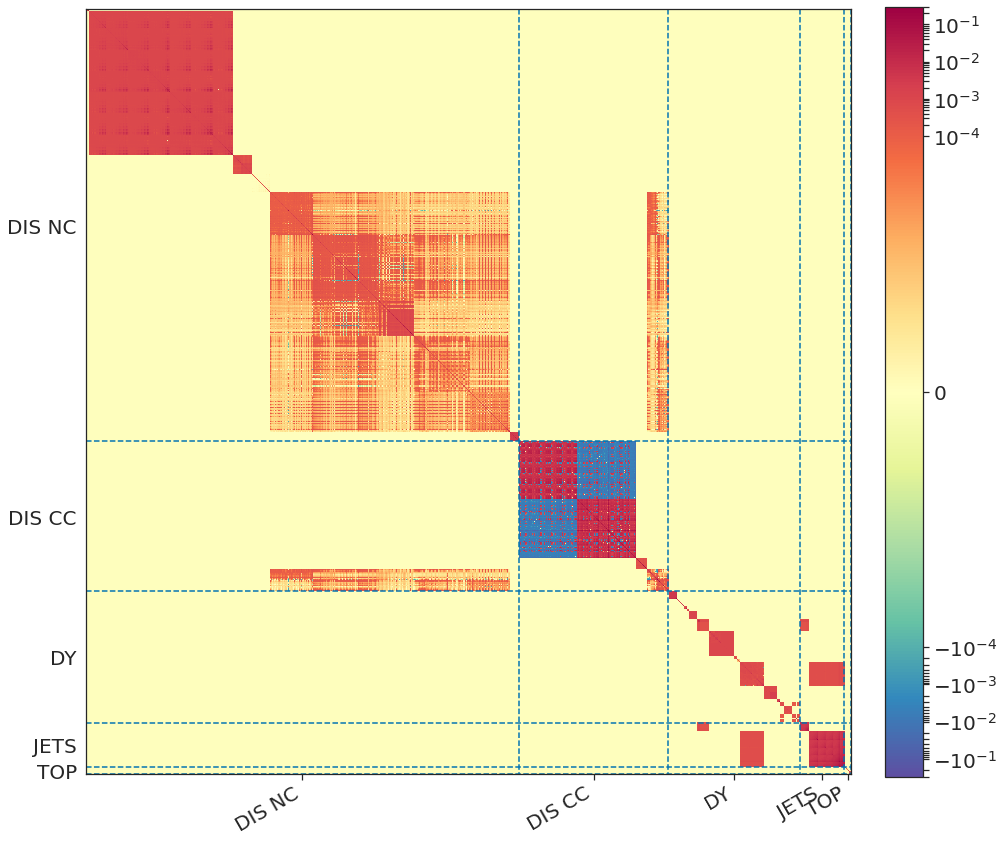
\includegraphics[width=0.48\columnwidth]{correlations/plots/C.png}}
\makebox{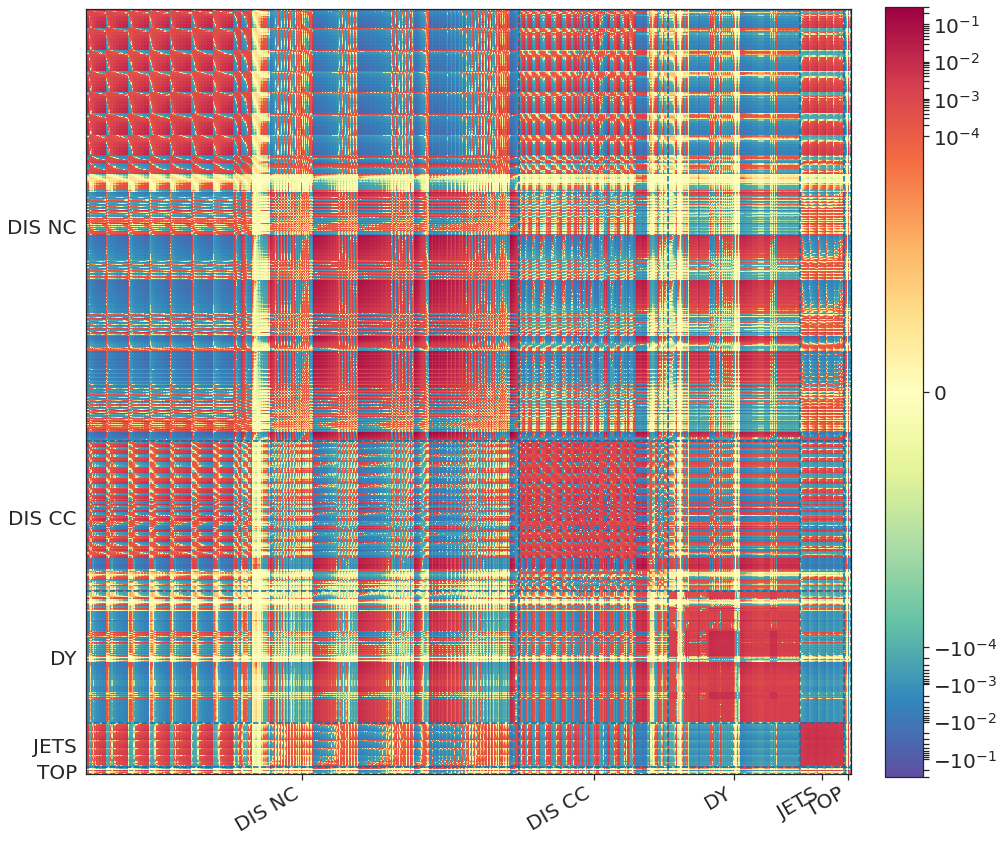
\includegraphics[width=0.48\columnwidth]{correlations/plots/S.png}}
    \end{center}
  \vspace{-0.55cm}
  \caption{The experimental covariance matrix, $C_{ij}$, normalised to the theoretical predictions $T^{(0)}_i$  (left), and the corresponding theory covariance matrix for MHOU, $S_{ij}$ (right). The datasets are arranged in the order given in Fig.~\ref{fig:chi2auto} below: so SLAC data are in the top left corner, and LHC top data in the lower right corner.}
  \label{fig:CnS}
\end{figure}
%%%%%%%%%%%%%%%%%%%%%%%%%%%%%%%%%%%%%%%%%%%%%%%%%%%%%%%%%%%%%%%%%%%%%%%%%%%%
 \begin{figure}[H]
    \begin{center}
    \makebox{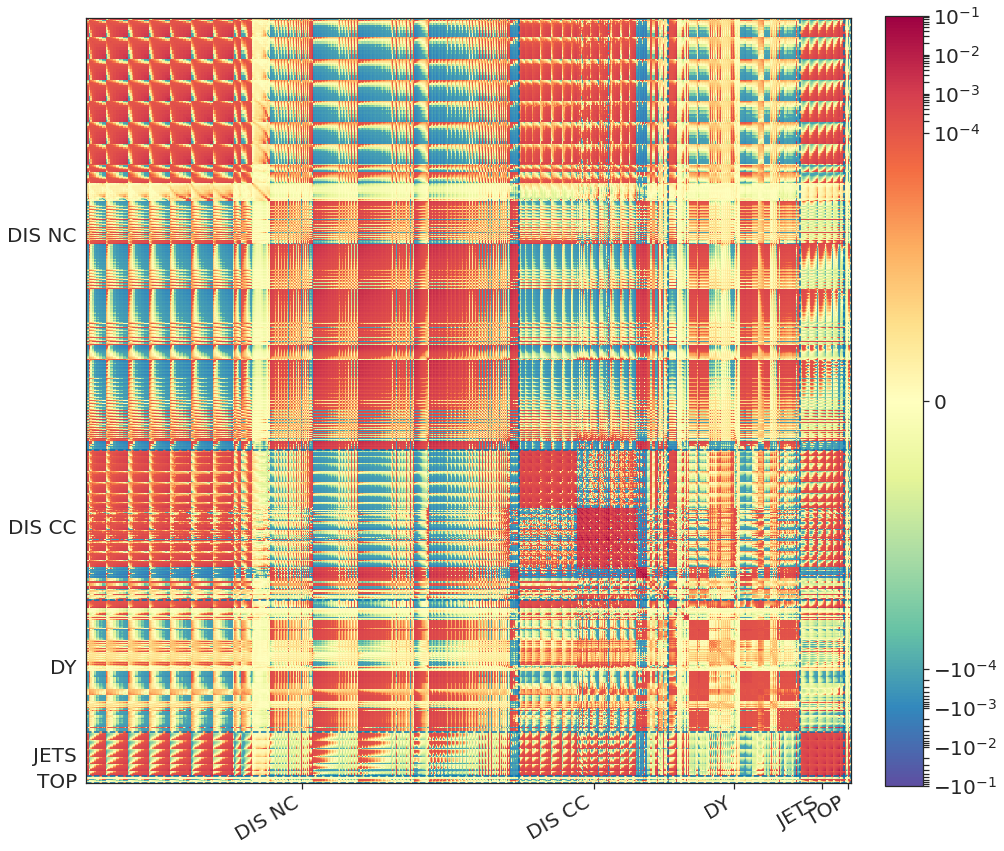
\includegraphics[width=0.48\columnwidth]{correlations/plots/X_covmat_cutscale.png}}
\makebox{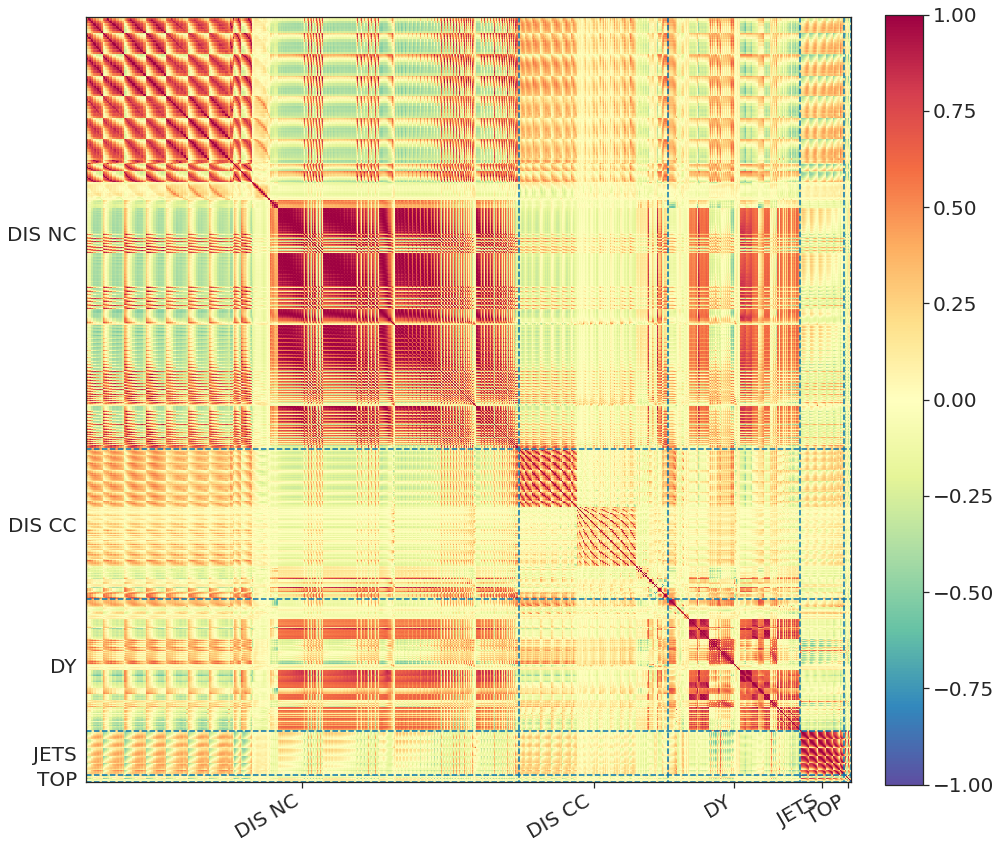
\includegraphics[width=0.48\columnwidth]{correlations/plots/Xcorrmat.png}}
    \end{center}
  \vspace{-0.55cm}
  \caption{The covariance matrix of PDF uncertainties, $X_{ij}$, normalised to the theoretical predictions $T^{(0)}_i$  (left), and the corresponding correlation matrix $X_{ij}/\sqrt{X_{ii}X_{jj}}$ (right). The datasets are arranged in the order given in Fig.~\ref{fig:chi2auto} below: so SLAC data are in the top left corner, and LHC top data in the lower right corner.}
  \label{fig:X}
\end{figure}
%%%%%%%%%%%%%%%%%%%%%%%%%%%%%%%%%%%%%%%%%%%%%%%%%%%%%%%%%%%%%%%%%%%%%
This is because theory predictions are often very strongly correlated, not only for nearby bins within the same experiment but also for different processes at nearby scales. This is primarily due to the smoothness of the underlying PDFs in $(x,Q^2)$, but it is also a consequence of the highly correlated theory uncertainties included in the fit.
 \begin{figure}[H]
    \begin{center}
    \makebox{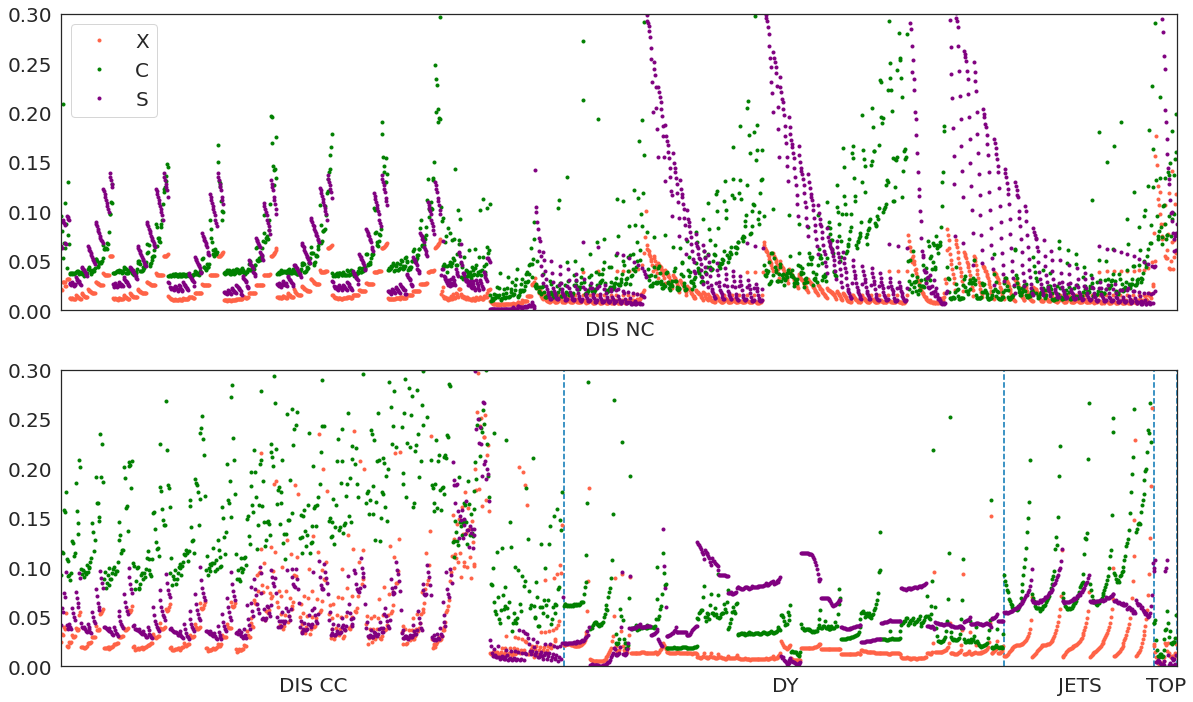
\includegraphics[width=0.99\columnwidth]{correlations/plots/CXS.png}}
    \end{center}
  \vspace{-0.55cm}
  \caption{The square root of the diagonal elements of the matrices $X$ (in orange), $C$ (in green) and $S$ (in purple) normalised to the theoretical predictions $T^{(0)}_i$, with those for $C$ and $S$ the same as in Chapter~\ref{chapter:mhous}. The datasets are arranged in the order given in Fig.~\ref{fig:chi2auto} below.}
  \label{fig:CXS}
\end{figure}
We compare PDF uncertainties to experimental and theory uncertainties by looking at the per-point uncertainty in Fig.~\ref{fig:CXS}. Recall from Eqn.~\ref{eq:repavD} that $C+S$ is the covariance of the data replicas to which the PDFs are fitted. At NLO, the relative size of $C_{ii}$ and $S_{ii}$ can vary quite  alot between datasets; for fixed target DIS, $S_{ii}$ is generally greater than $C_{ii}$, except at large $x$. For HERA NC there is an interesting pattern whereby $S_{ii} \ll C_{ii}$ at large $x$, but the opposite is true at small $x$. The experimental uncertainty is also dominant for CHORUS, but for most of DY the theory uncertainty dominates. 

The PDF uncertainties, $X_{ii}$ are generally less than both the experimental and theoretical uncertainties. This makes sense because they are the product of a fit, and so the uncertainty on each point is influenced by all the other data points in the fit, which collectively conspire to reduce the uncertainty. We can clearly see this effect in DY and JETS. The exception to this are datasets with very small theory uncertainty, for example ratio datasets where systematic uncertainties cancel between the numerator and denominator (e.g. NMC $d/p$, asymmetry data and differential top). In these instances, $X_{ii}$ is above $S_{ii}$, though still lower than $C_{ii}$.

\subsection{Nuisance parameters} 
Now let's look at the nuisance parameters $\lambda_\alpha$ of the covariance matrix $S$. We showed in Chapter \ref{chapter:mhous} that for five processes in the 9 point prescription there are 28 non-zero eigenvalues, and so we will have 28 nuisance parameters. Fig.~\ref{fig:nuisancediag} shows these eigenvalues in descending order in the top panel, with their nuisance parameters below. We computed the expectation value of the nuisance parameters using Eqn.~\ref{eq:shiftmult}, and their uncertainties using Eqn.~\ref{eq:Zbardefab}. 
It helps to separate out the two contributions to the uncertainty on the nuisance parameters, namely:
\begin{enumerate}
\item the scale uncertainty (Eqn.~\ref{eq:Zdefab});
\item the PDF uncertainty (last term in Eqn.~\ref{eq:Zbardefab}).
\end{enumerate}
These are shown as the lower two panels in Fig.~\ref{fig:nuisancediag}. 

Recall that the prior for the nuisance parameters was a unit Gaussian centred on zero (Eqn.~\ref{eq:priorf}). After fitting, we see that the total uncertainty in the nuisance parameters for the largest $\sim$9 eigenvalues has been substantially reduced, showing that the MHOU along these directions has been learnt in the fitting process. For the nuisance parameters corresponding to the smaller eigenvalues there is very little reduction. This tells us that the data don't constrain these directions very well. The central values for the largest three eigenvalues are very close to zero within uncertainties. This shows that the choice of prior was reasonable. The next three or so significantly deviate from zero, showing that the data must have significant information about the MHOUs in these directions. For the remaining smaller eigenvalues, the central values of the nuisance parameters are all compatible with zero. For the very small ones it seems the data have had no effect at all because the posterior distributions are the same as the prior. So only the largest eigenvalues are actually relevant for PDF determination, and the others are simply ignored by the fit.

Looking now at the split between scale uncertainty and PDF uncertainty, we see that the MHOU for the largest eigenvalues is reduced a lot, showing that it is learnt in the same way we saw in the simple models of Secs~\ref{sec:p1}-\ref{sec:p3}. However, there is very little information extracted about the smaller ones. The PDF uncertainty is also small for the largest and smallest eigenvalues, but dominates for the middle ones. 
%%%%%%%%%%%%%%%%%%%%%%%%%%%%%%%%%%%%%%%%%%%%%%%%%%%%%%%%%%%%
  \begin{figure}[H]
    \begin{center}
    \makebox{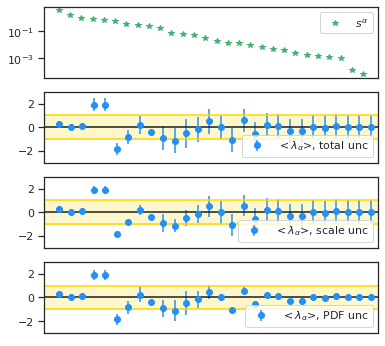
\includegraphics[width=0.7\columnwidth]{correlations/plots/lambdas.png}}
    \end{center}
  \vspace{-0.55cm}
  \caption{The $28$ positive eigenvalues $s^\alpha$ of the theory uncertainty matrix $S_{ij}$ (above), shown in descending order, and 28 nuisance parameters $\lambda_\alpha$ corresponding to the $28$ eigenvectors $\beta_\alpha$ (below), as given by Eqn.~\ref{eq:Elambdaf}.The uncertainties in the nuisance parameters are shown in total (square roots of the diagonal entries of Eqn.~\ref{eq:Zbardefab}, and broken down into the contribution from scale uncertainties alone (square roots of the diagonal entries of Eqn.~\ref{eq:Zdefab}  and from PDF uncertainties (square roots of the diagonal entries of the last term in Eqn.~\ref{eq:Zbardefab}. The yellow bands highlight the region between $\pm 1$.}
  \label{fig:nuisancediag}
%\end{figure}
 %\begin{figure}[h!]
    \begin{center}
    \makebox{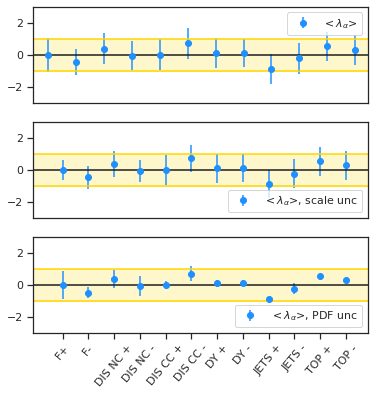
\includegraphics[width=0.55\columnwidth]{correlations/plots/lambdas_phys.png}}
    \end{center}
  \vspace{-0.55cm}
  \caption{Nuisance parameters $\lambda$ for directions in the space of scale variations corresponding to up/down changes in factorization scale, and in renormalization scale for the five types of processes in the determination of the $9$-pt theory covariance matrix for MHOU. The uncertainties in the nuisance parameters are shown in total, and broken down into the contribution from scale uncertainties alone and from PDF uncertainties, just as in Fig.~\ref{fig:nuisancediag}. The yellow bands highlight the region between $\pm 1$.}
  \label{fig:nuisancephys}
\end{figure}
%%%%%%%%%%%%%%%%%%%%%%%%%%%%%%%%%%%%%%%%%%%%%%%%%%%%%%%%%%%%

Having seen that some directions of MHOU are more relevant in the fit, we may wonder whether these have a physical interpretation; in Fig.~\ref{fig:evecs1} of Chapter \ref{chapter:mhous} we saw that the largest eigenvectors of $S$ were driven by factorisation scale variation and then renormalisation scale variation for DIS NC. To investigate this, we can switch bases, choosing $\beta_\alpha$ to correspond to factorisation scale variations (up/down) and renormalisation scale variations (up/down for each process). Fig.~\ref{fig:nuisancephys} is a similar plot to Fig.~\ref{fig:nuisancediag}, but for this ``physical" basis. 

We see that the central values fluctuate about zero, but stay in the $\pm$1 band, showing again that the impact of fitting the data on the nuisance parameters is not large. This is reassuring as it backs up the choice of central scales and the choice of range of scale variations (the latter being implicit in the prior for $\lambda_\alpha$). Looking just at the scale uncertainty, it is apparent that the factorisation scale variation nuisance parameters have learnt the most information, which makes sense as factorisation scale variation is common to all data in the fit. NC DIS, being the largest process, is also learnt about to some extent. However, including the PDF uncertainty washes out these effects. In particular, the uncertainties in these directions can be slightly greater than one in total; in fact there is less learnt about the factorisation scale nuisance parameters that we had supposed in the prior.

Already we see that information from the data in the fit significantly updates the priors for the nuisance parameter distribution. From this it is likely that there will be an effect at the level of the autopredictions, which is the subject of the next section.

\subsection{Autopredictions}
\label{subsec:autopredictions}
As described in Sec.~\ref{sec:p1}, autopredictions are where we fit a PDF and then use that PDF to make predictions for the data that went into the PDF. These are essentially postdictions, and are ideal for testing the extent of correlation between theory uncertainties in the PDF fit and in the (auto)predictions. 

Although this situation is somewhat artificial because experiments are never redone in exactly the same way, the implications of this investigation will be general. This is because for a global fit of this size (2819 data points, 35 datasets and 5 processes), removing only one of the smaller datasets has negligible impact on the PDFs. 
%%%%%%%%%%%%%%%%%%%%%%%%%%%%%%%%%%%%%%%%%%%%%%%%
\begin{figure}[H]
    \begin{center}
    \makebox{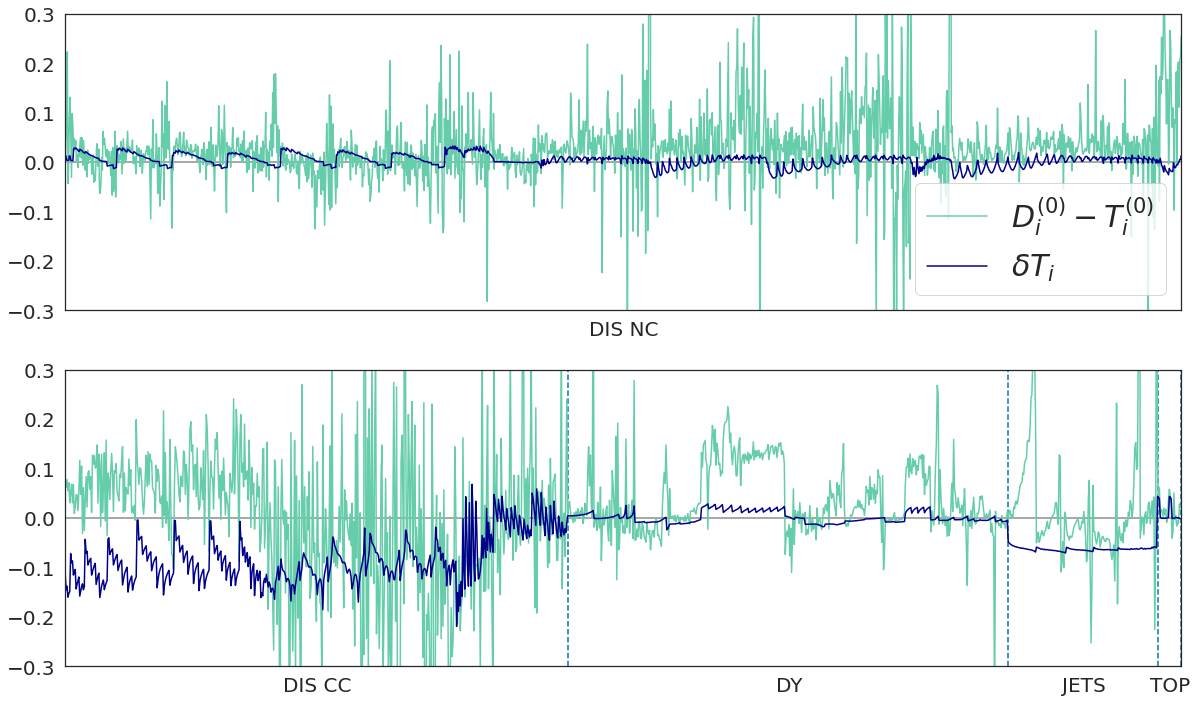
\includegraphics[width=0.95\columnwidth]{correlations/plots/shifts.png}}
    \end{center}
  \vspace{-0.55cm}
  \caption{The shifts $\delta T_i$, Eqn.~\ref{eq:shiftNN} (in blue) compared to the differences between theory and data, $D_i-T^{(0)}_i$ (in green), both normalised to $T^{(0)}_i$.} 
  \label{fig:shifts}
\end{figure}
%%%%%%%%%%%%%%%%%%%%%%%%%%%%%%%%%%%%%%%%%%%%%%%%%%
Removing even a large dataset will only increase PDF uncertainties without affecting the theory uncertainties for the remaining data. This means that if we did the fit with a certain dataset removed, and did the analysis with that fit instead, we would instead have a genuine prediction, and the correlations between MHOUs in the PDF and the prediction would be very close to what we have for the autopredictions.

To make the correlated autopredictions, we first compute $\delta T_i$ (Eqn.~\ref{eq:shiftmult}). This is the shift in theory predictions arising due to theory correlations. We show this in Fig.~\ref{fig:shifts}, normalised to the orginal theoretical prediction $T^{(0)}_i$. We also show $D_i-T_i^{(0)}$ for comparison. The shifts tend to be small, however for some datasets (especially CHORUS and inclusive jets) there is a systematic overall shift of order $D_i-T_i^{(0)}$.

\begin{table}[b!]
\centering
\begin{tabular}{|l||ccccc|c|}
\hline
                   & \textbf{DIS NC} & \textbf{DIS CC} & \textbf{DY} & \textbf{JETS} & \textbf{TOP} & \textbf{Total} \\
                   \hline
No th uncs         & 1.13            & 0.98            & 1.56        & 0.88         & 1.20         & 1.17           \\
Uncorr th uncs     & 1.15            & 1.06            & 1.53        & 0.90         & 1.27         & 1.19           \\
Correlated th uncs & 1.09            & 0.91           & 1.47        & 0.83         & 0.97        & 1.10    \\
\hline
\end{tabular}
\vspace{1cm}
\caption{The experimental $\chi^2$ per data point for each process, comparing the original result of the NLO fit with no theory uncertainties to the fit with theory uncertainties, and then including the shift in the autopredictions.}
  \label{tab:chisq}
\end{table}

It's interesting to see whether the shifts improve the autopredictions. In Fig.~\ref{fig:chi2auto} we show the $\chi^2$ of the autopredictions, using the experimental covariance matrix only, for the following autoprediction central values:
\begin{itemize}
\item No theory uncertainty;
\item Theory uncertainty in the fit;
\item Shifted autopredictions.
\end{itemize}
\begin{figure}[H]
    \begin{center}
    \makebox{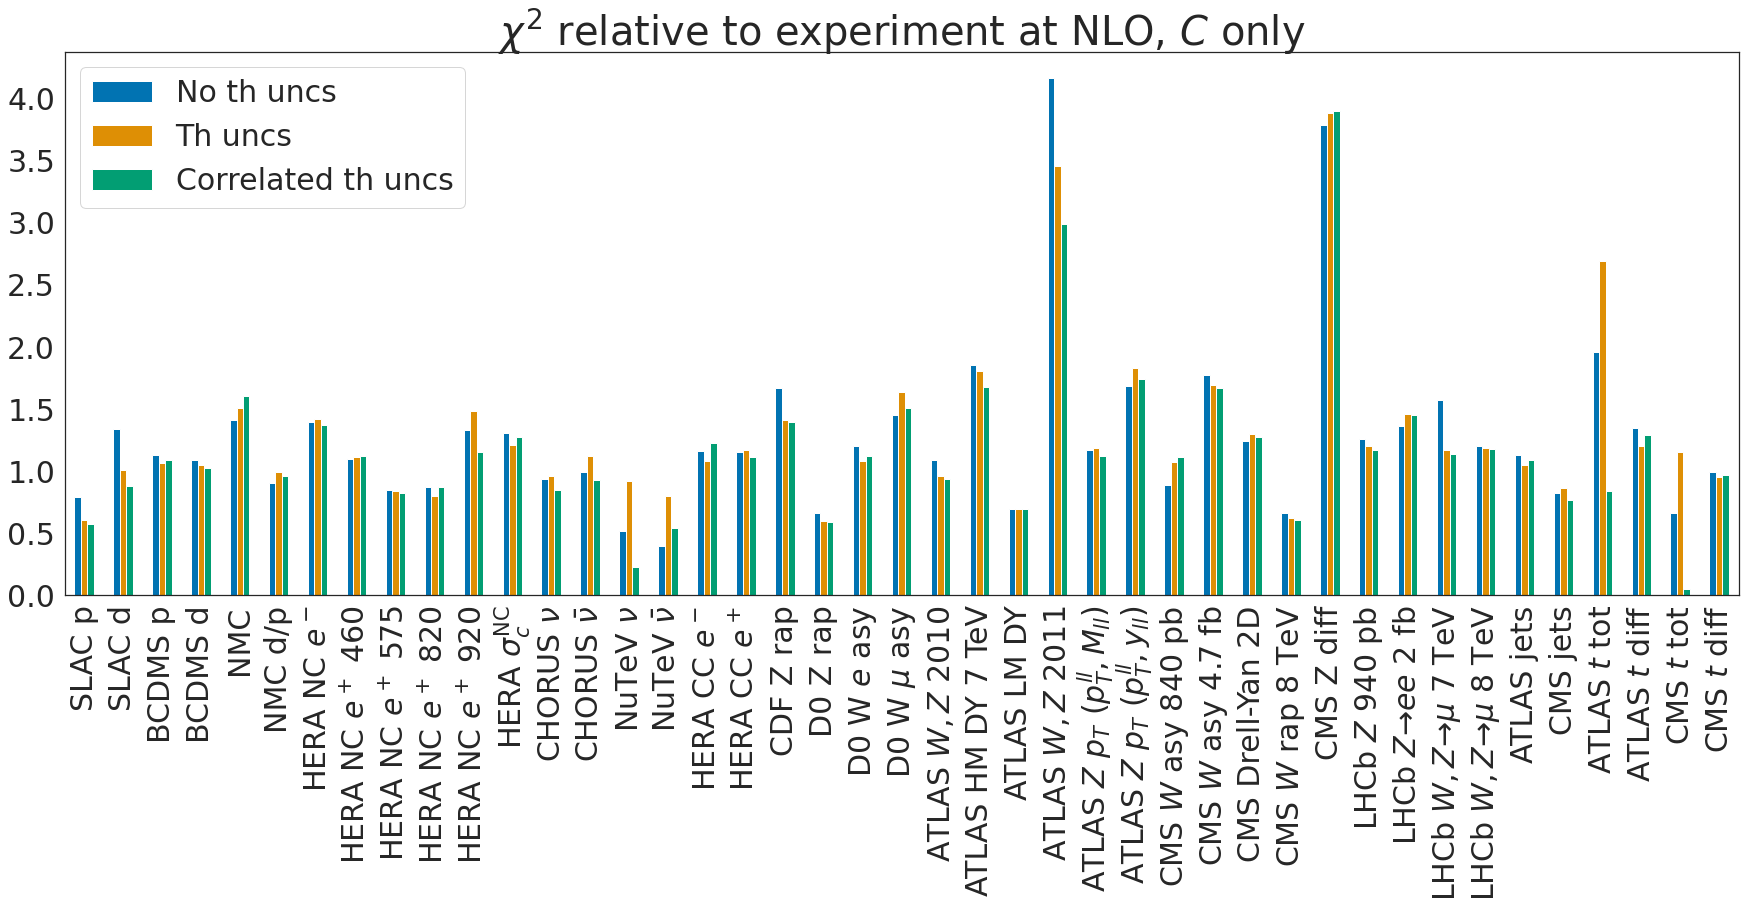
\includegraphics[width=0.99\columnwidth]{correlations/plots/chi2_auto.png}}
    \end{center}
  \vspace{-0.55cm}
  \caption{The experimental $\chi^2$ for each data set, comparing the original result of the NLO fit with no theory uncertainties to the fit with theory uncertainties, and then including the correlated shift in the autopredictions.}
  \label{fig:chi2auto}
\end{figure}
We use only the experimental covariance matrix, in order to isolate the effects due to the changing central value from those due to adding additional uncertainties. 

The results for all cases are very similar. Including the theory uncertainty in the fit has mixed results; some predictions get better at the expense of others getting worse. This is because the main effect of including theory uncertainties is to rebalance the fit. When the correlated shift is also included, the fit to most datasets improves, in some cases substantially. The exact values are broken down by process in Tab.~\ref{tab:chisq}. When including theory uncertainties, the $\chi^2$ goes up slightly from 1.17 to 1.19. However, when the correlated shift is added, there is a significant improvement across all processes, with the total $\chi^2$ dropping to 1.10.

\begin{figure}[H]
    \begin{center}
    \makebox{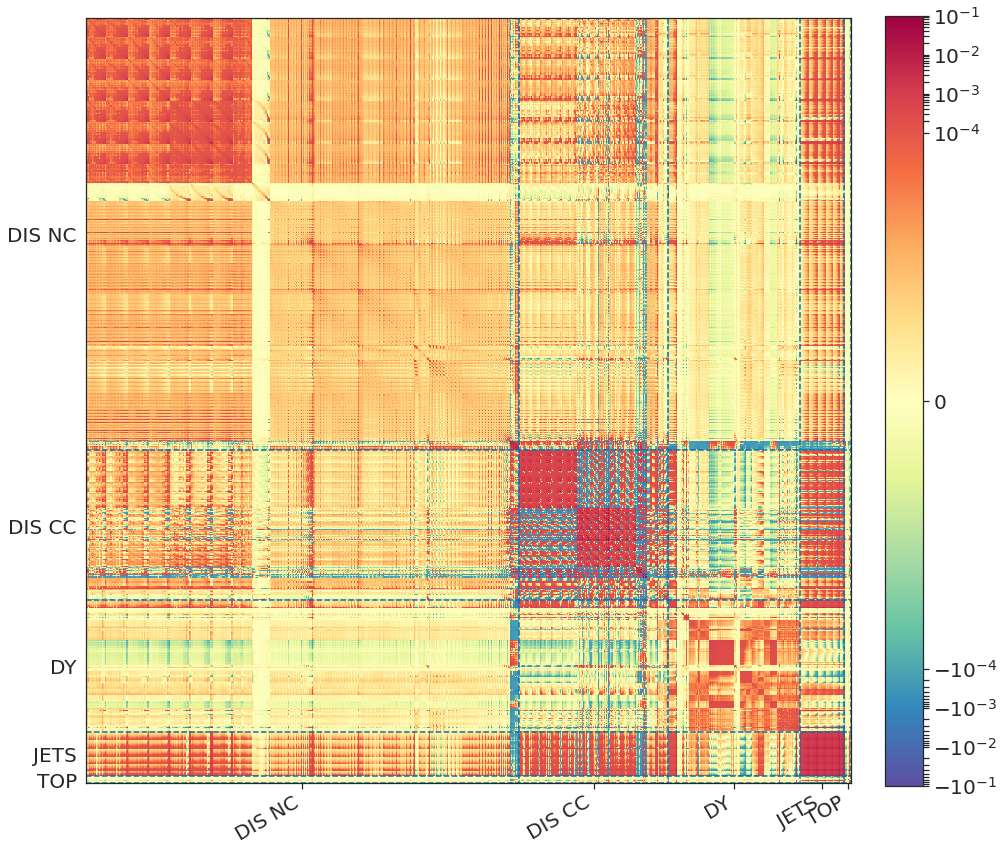
\includegraphics[width=0.48\columnwidth]{correlations/plots/P.png}}
    \makebox{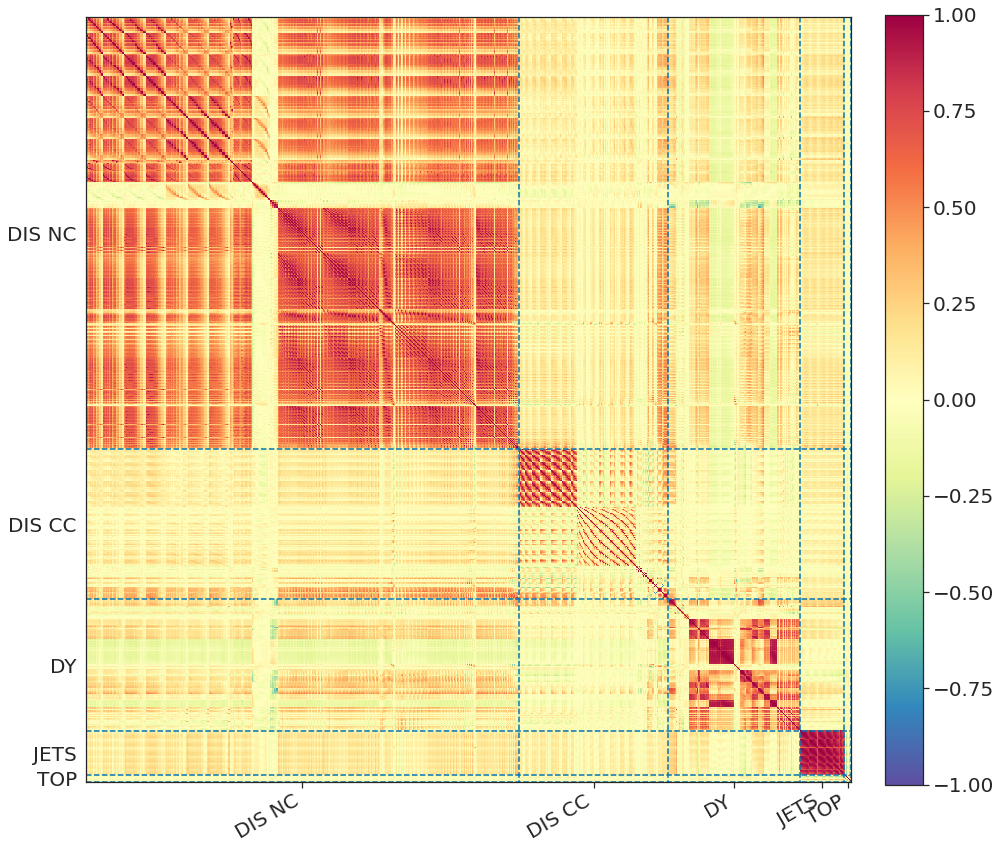
\includegraphics[width=0.48\columnwidth]{correlations/plots/P_corrmat.png}}  
  \end{center}
  \vspace{-0.55cm}
  \caption{The autoprediction covariance matrix $P_{ij}$ Eqn.~\ref{eq:PNN}, normalised to the theoretical predictions $T^{(0)}_i$ (left), and the corresponding corrrelation matrix $P_{ij}/\sqrt{P_{ii}P_{jj}}$ (right).}
  \label{fig:P}
%\end{figure}
%\begin{figure}[t!]
    \begin{center}
    \makebox{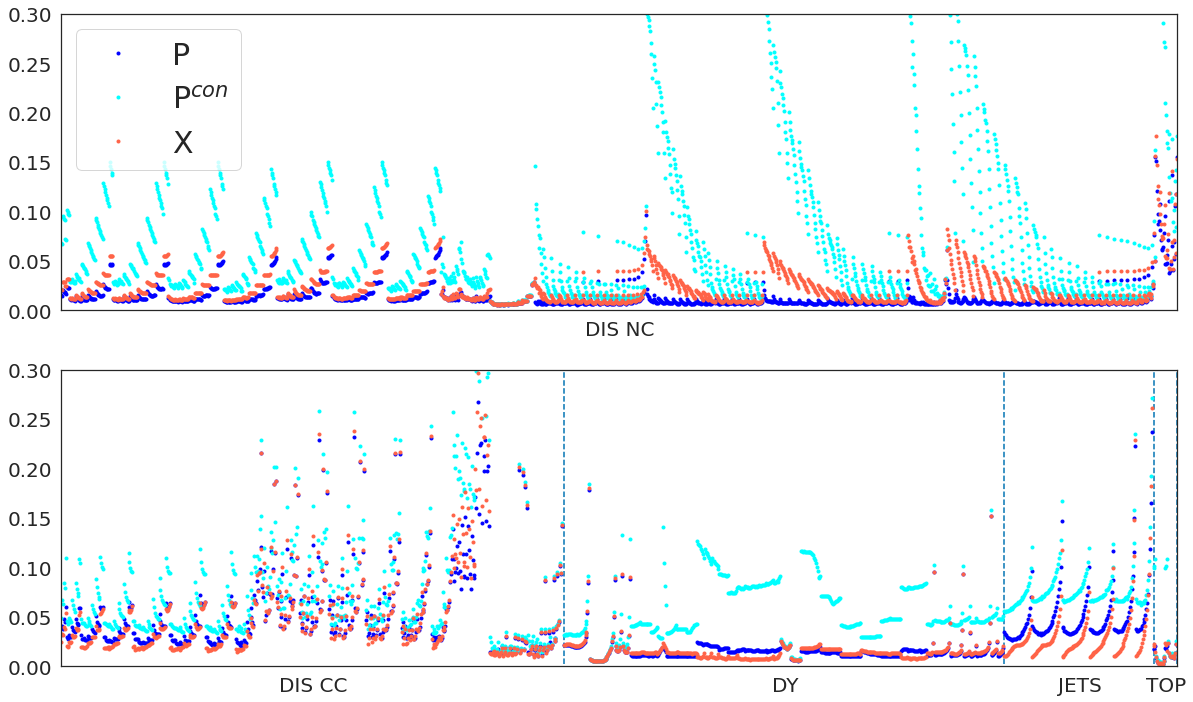
\includegraphics[width=0.99\columnwidth]{correlations/plots/XPPcon.png}}
    \end{center}
  \vspace{-0.55cm}
  \caption{The percentage uncertainties of the autopredictions $\sqrt{P_{ii}}$ Eqn.~\ref{eq:PNN} (cyan) compared to the PDF uncertainty $\sqrt{X_{ii}}$ (orange),  and the conservative result, $\sqrt{P^{\rm con}_{ii}}$ Eqn.~\ref{eq:PconNN} (dark blue), all normalised to the theoretical predictions $T^{(0)}_i$.}
  \label{fig:Pdiag}
\end{figure}

Now let's see whether we also end up with an increase in precision, by considering the uncertainties in the autopredictions. In Fig.~\ref{fig:P} we show the full covariance matrix of autopredictions normalised to theory predictions and also as a correlation matrix. Remember that $P_{ij}$ is the sum of:
\begin{enumerate}
\item The PDF uncertainty, derived from a combination of the experimental and theory uncertainties in the fit;
\item The theory uncertainty in the autoprediction.
\end{enumerate}
Each of these contributions is reduced due to the learning of the theory uncertainties and the correlation between the two sources of theory uncertainty. As might be expected, we can see that there are very large correlations in the autopredictions within datasets. These are due to:
\begin{enumerate}
\item Correlation of experimental uncertainties within datasets;
\item Smooth underlying PDFs;
\item Correlations of theory uncertainties.
\end{enumerate}
Correlations are generally larger within each process than outwith them. This suggests that the factorisation scale correlation is small compared to the combination of the renormalisation scale correlation and the effects from PDF smoothness and experimental uncertainties.

Fig.~\ref{fig:Pdiag} shows the percentage uncertainties of the autopredictions, $\sqrt{P_{ii}}/T_i$, compared to the original PDF uncertainties, $\sqrt{X_{ii}}/T_i$. It also shows the percentage uncertainties for the conservative prescription, $\sqrt{P^{con}_{ii}}/T_i$. The correlated autoprediction uncertainties are generally a similar size to the PDF uncertainties. They are larger for some of the DY datasets and JETS, and for most of DIS NC and some DY they are smaller. This is in stark contrast to the uncorrelated conservative prescription, which are greater than the PDF uncertainties across the board, sometimes by a lot, and typically a factor of two or more. This is because they don't take into account the correlation or the learning, which leads to an overestimate, especially where the theory uncertainties are a lot bigger than the PDF uncertainty. In fact, the conservative prescription only works well where the theory uncertainties are very small, for example the NMC $d/p$ ratio data. 

The upshot is that the correlated autopredictions are not only more accurate, they are also more precise. But we do need to be wary of this increase in precision because it depends implicitly on the assumptions made when modelling the prior MHOUs that we made in Chapter \ref{chapter:mhous}. In particular, it is dependent on the choice of independent scales, the size of variation, and the prescription for generating $S$. For example, the aggressive reduction in small $x$ uncertainty for HERA NC may well be due to the unseparated singlet and non-singlet factorisation scale variation; because of this the singlet evolution is overconstrained at small $x$~\cite{Harland-Lang:2018bxd}. We leave this as a matter for future work.

\begin{figure}[H]
    \begin{center}
    \makebox{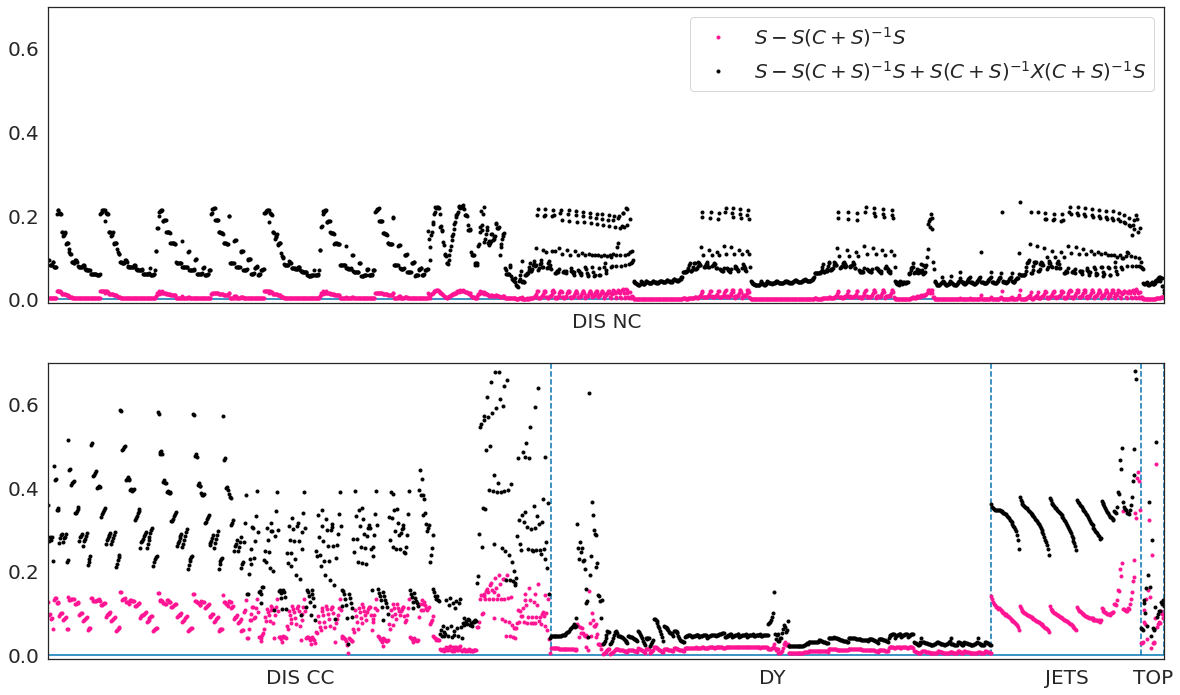
\includegraphics[width=0.99\columnwidth]{correlations/plots/split_th.png}}
    \end{center}
  \vspace{-0.55cm}
  \caption{The contributions to the diagonal elements of the correlated theory uncertainty normalised to diagonal elements of S: $(S-S(C+S)^{-1}S)_{ii}/S_{ii}$ (pink), and  $(S-S(C+S)^{-1}S+S(C+S)^{-1}X(C+S)^{-1}S )_{ii}/S_{ii}$ (black).}
  \label{fig:Scpts}
\end{figure}

To understand better how these changes in uncertainty arise, we show in Fig.~\ref{fig:Scpts} a breakdown of the diagonal elements of the correlated theory uncertainty (the second term in Eqn.~\ref{eq:PNN}), normalised to the theory uncertainty prior, $S_{ii}$. Explicitly, the contributions are 
\be 
S - S(C+S)^{-1}S + S(C+S)^{-1} X(C+S)^{-1} S.
\ee
The first term is the prior, the second term is due to learning, and the third term is due to PDF fluctuations. Note that the first two terms are $ZS$ and the whole expression is $\Zbar S$ in the one parameter model. 

We can see that the learning reduces the prior almost to zero for NC DIS and DY, and by an order of magnitude for the rest. It is likely that more flexibility is required in the prior. The PDF fluctuations then undo a lot of the learning, but the overall uncertainty is still less than the prior.

We can do a similar breakdown for the correlated PDF uncertainty diagonals, this time normalised to $X_{ii}$. This is the first term in Eqn.~\ref{eq:PNN}, but expanded out like in Eqn.~\ref{eq:Xalgebra2}. The correlation terms, $-S(C+S)^{-1}X-X(C+S)^{-1}S$, are very large as anticipated in \cite{Harland-Lang:2018bxd}. This is especially true where there is a large theory uncertainty (small $x$ HERA NC or JETS), and here they can overwhelm $X$ and give a negative result. Despite that, the addition of PDF fluctuations in $S(C+S)^{-1}X(C+S)^{-1}S$ (rememeber the breakdown in Eqn.~\ref{eq:Xalgebra2}) always leaves the total positive, sometimes taking it higher than $X$. We can therefore see that adding correlations generally reduces the uncertainties, but they can sometimes increase them. The learning, however, always reduces them.
\begin{figure}[H]
    \begin{center}
    \makebox{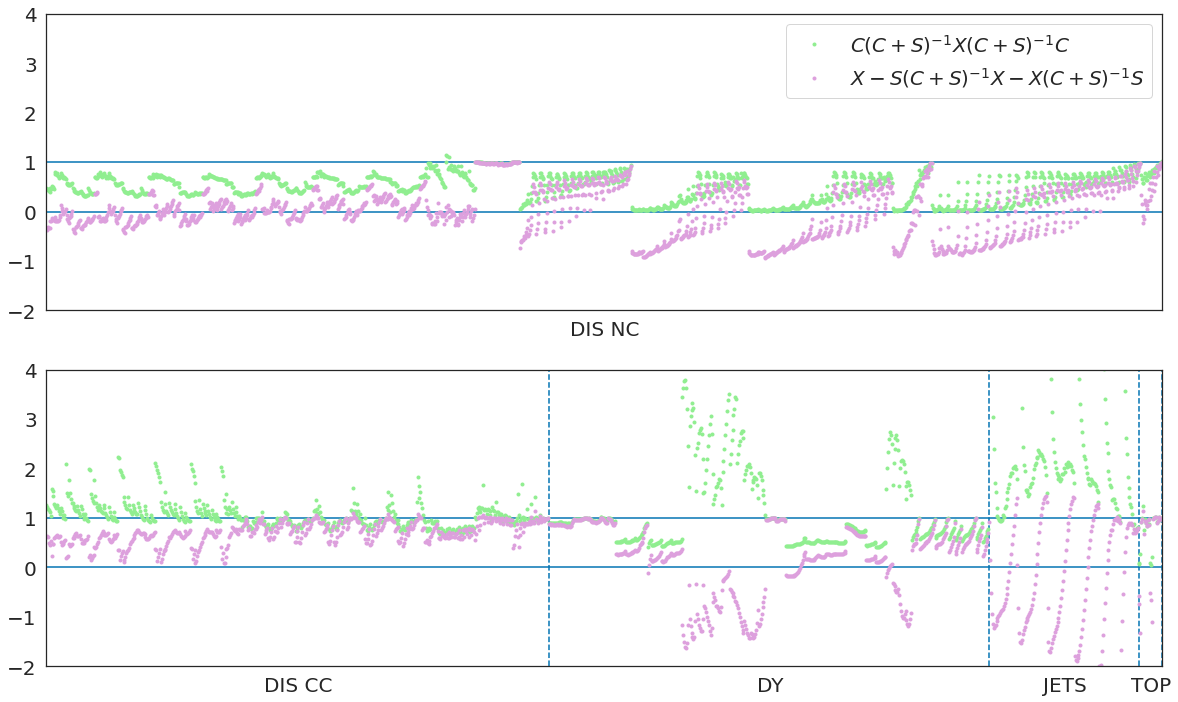
\includegraphics[width=0.99\columnwidth]{correlations/plots/split_pdf.png}}
    \end{center}
  \vspace{-0.55cm}
  \caption{The contributions to the diagonal elements of the correlated PDF uncertainty normalised to diagonal elements of X: $(X-S(C+S)^{-1}X-X(C+S)^{-1}S)_{ii}/X_{ii}$ (lilac), and  $(C(C+S)^{-1}X(C+S)^{-1}C )_{ii}/X_{ii}$  (see Eqn.~\ref{eq:Xalgebra2} (green).}
  \label{fig:Xcpts}
\end{figure}
For the autopredictions, we expect high levels of learning and correlation, because we are making predictions for exact repetitions of experiments already in teh fit. However, as noted earlier, removing one of the smaller datasets will have little effect on the fit, which leads us to suspect that there will be similar results for genuine predictions if the process is already in the fit and, especially, if the kinematics are similar.

\subsection{Predictions for an existing process: top production}
\label{subsec:topnhiggs}
Finally we can consider genuine predictions for experiments that weren't used in the PDF fits. These can either be for processes already in the fit, or for new ones. Here we consider the former, and in the next subsection we'll end with the latter.
\begin{figure}[H]
    \begin{center}
    \makebox{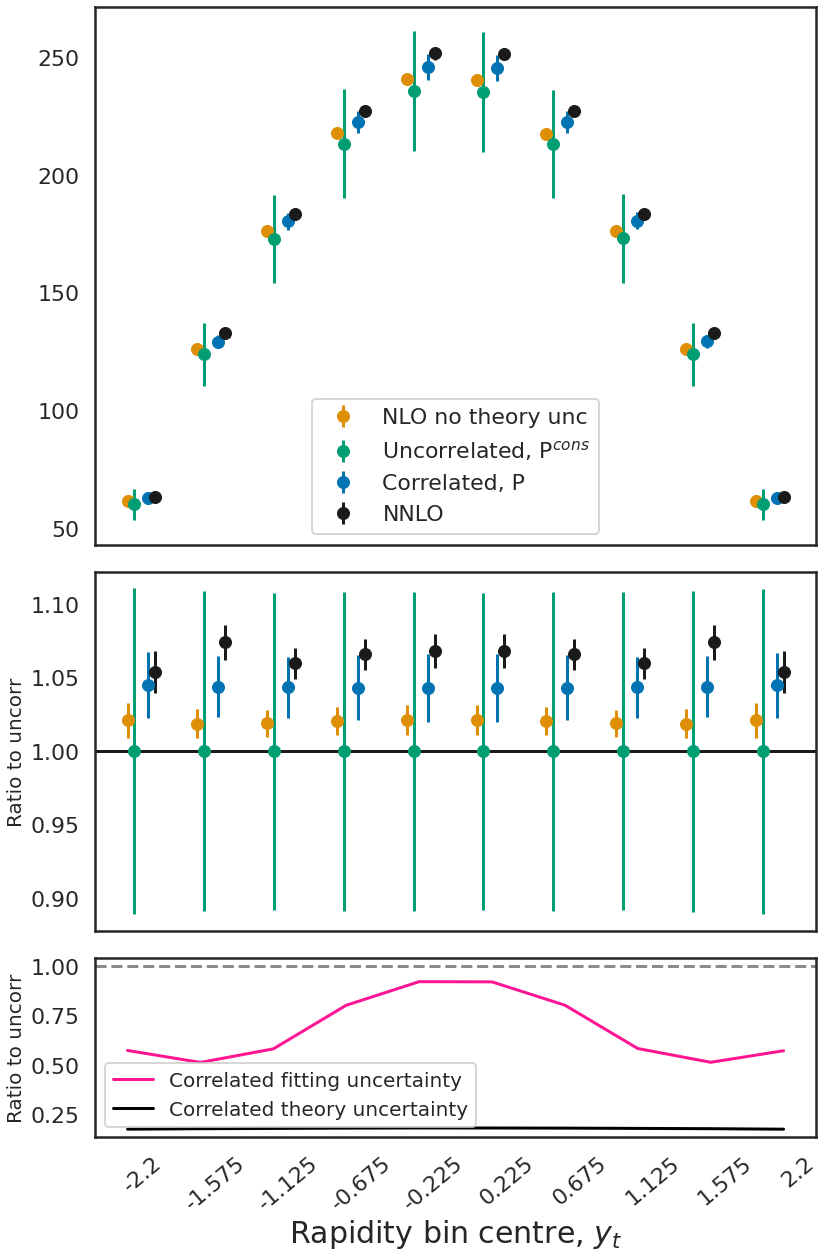
\includegraphics[width=0.46\columnwidth]{correlations/plots/topdilepton.png}}
   \makebox{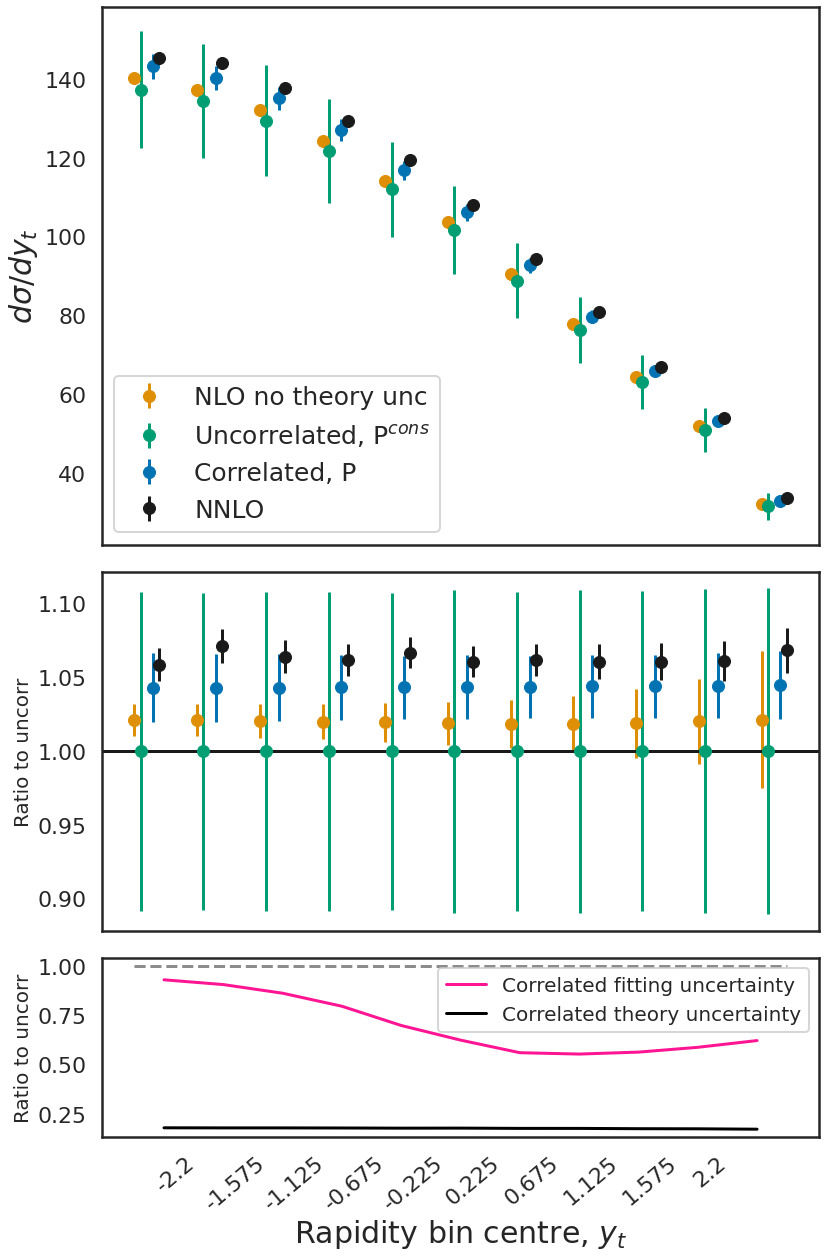
\includegraphics[width=0.46\columnwidth]{correlations/plots/toplj.png}}
    \end{center}
  \vspace{-0.55cm}
  \caption{The upper two panels show predictions for $t\bar{t}$ unnormalised rapidity distribution data taken at 13~TeV by CMS, the dilepton rapidity distribution \cite{Sirunyan:2018ucr} (left) and the lepton+jets distribution \cite{Sirunyan:2018wem} (right). The four predictions show: the NLO fit with no MHOUs, PDF error only; the combined PDF and MHOU fit, ignoring correlations (thus $\sqrt{P_{II}^{\rm con}}$); the result with the same shift, but with the correlations included exactly (thus $P_{II}$), and the NNLO result with no MHOU. In the middle panels the same is shown, but normalised to the uncorrelated result. In the lower panels we show the fractional reduction in the PDF uncertainty and the theory uncertainty due to the inclusion of the correlations.}
  \label{fig:CMSttbar}
\end{figure}

We look at $t\bar{t}$ production rapidity distributions in two channels (dilepton and lepton + jets), measured by CMS at 13 TeV~\cite{Sirunyan:2018ucr,Sirunyan:2018wem}. There are a couple of reasons for this choice:
\begin{itemize}
\item The base fit contains $t\bar{t}$ total cross sections at 7, 8 and 13 TeV and normalised rapidity distributions at 8 TeV, all from both ATLAS and CMS.
\item The NLO theory uncertainty for the 13 TeV data is $\sim$10\%, considerably larger than the PDF uncertainty.
\end{itemize}
Both these things mean that we'd expect the correlation between the theory uncertainties in these data and the 13 TeV distributions to be high, and so we should see some of the largest effects currently possible with these PDFs. The CMS 13 TeV $t\bar{t}$ rapidity predictions were computed using the same procedure as the 8 TeV distributions in \cite{Ball:2017nwa}: NLO theoretical predictions were generated with {\tt Sherpa}~\cite{Gleisberg:2008ta}, in a format compliant with {\tt APPLgrid}~\cite{Carli:2010rw}, using the {\tt MCgrid} 
code~\cite{DelDebbio:2013kxa} and the {\tt Rivet}~\cite{Buckley:2010ar} analysis package, with {\tt OpenLoops}~\cite{Cascioli:2011va} for the NLO 
matrix elements. Renormalisation and factorisation scales have been chosen based on the recommendation of \cite{Czakon:2016dgf} as $H_T/4$.

The predictions are shown in Fig.~\ref{fig:CMSttbar}. The correlated shift is sizeable, about 5\%, but this is still comfortably within the $\sim$10\% theory uncertainty. We'd anticipate this given that Fig.~\ref{fig:nuisancephys} tells us that the shift in nuisance parameters for the top renormalisation scale variation is also well within uncertainties. We also see that the shift is almost fully correlated across the whole distribution. This is because these are unnormalised distributions, so there is the restriction that they must sum to the total cross section. They are therefore strongly correlated with the measurements of the total cross section in the fit. We can confirm this by breaking down the contributions to the shift from the different fitted data points, seen in Table ~\ref{tab:deltilcons}. The six total cross section measurements are responsibile for the vast majority of the shift, with the 8 TeV normalised rapidity distributions pushing the shift back down by about 25\%. The rest of the data have almost no impact.
%%%%%%%%%%%%%%%%%%%%%%%%%%%%%%%%%%%%%%%%%%%%%%%%%%%%%%%%%%%%%%%%%%
\begin{table}[h]
  \centering
  \scriptsize
  \renewcommand{\arraystretch}{1.4}
  \begin{tabular}{|llll|llll|l|}
   \hline
 {\bf ATLAS} &&&& {\bf CMS} &&&& {\bf Other}\\
 {\it tot} &&&{\it diff} &{\it tot}&&&{\it diff} & \\
  7 TeV &  8 TeV & 13 TeV & 8 TeV &7 TeV & 8 TeV &13 TeV & 8 TeV & \\
    \hline
 0.37 & 0.11 & 0.24 & -0.21 & 0.26 & 0.21 & 0.07 & -0.04 & -0.01 \\
\hline
  \end{tabular}
\caption{The fractional contributions of different data sets included in the fit to the
shifts in the top rapidity distributions, averaged over all 21 data points.}
\label{tab:deltilcons}
\end{table}
%%%%%%%%%%%%%%%%%%%%%%%%%%%%%%%%%%%%%%%%%%%%%%%%%%%%%%%%%%%%%%%%%%

To see if the shift improves the predictions, we can compare it to the known NNLO-NLO shift, just like we did in Chapter ~\ref{chapter:mhous}. Therefore, in Fig.~\ref{fig:CMSttbar} we also show the full NNLO result (without theory uncertainties). It's interesting that the shift due to correlations, which we saw is driven by the $t\bar{t}$ total cross section data, largely accounts for the NNLO correction; the data know that the NLO theory predictions are a bit low, and that knowledge is propagated into the predictions for the 13 TeV rapidity distributions. 

In terms of the change in uncertainties, the middle panels show the same as the top panels but as a ratio to the uncorrelated case, making the uncertainties more visible. Comparing the difference between the uncorrelated and correlated is striking; the correlated uncertainties are far smaller than the uncorrelated ones. However, despite substantial reduction of the very large theory uncertainty, they are still larger than the pure PDF uncertainties. Even though the uncertainties have shrunk a lot, they are still compatible with the NNLO result thanks to a shift in the central values. While the conservative prescription is also compatible with the NNLO result, it is immediately obvious from the plot that it is inferior. 

A breakdown of the reduction in uncertainties due to the correlations is shown in the bottom panels of Fig.~\ref{fig:CMSttbar}. The correlated theory uncertainty is substantially reduced (uniformly across rapidity). This is due to the learning of the normalisation from the data already in the fit. The correlated PDF uncertainty is reduced a lot less, maximally a factor of two for where the cross section is small, but hardly at all where the cross section is large. From this it is clear that the dominant effect here is the learning of the theory uncertainty in the overall normalisation.

\begin{figure}[h]
    \begin{center}
    \makebox{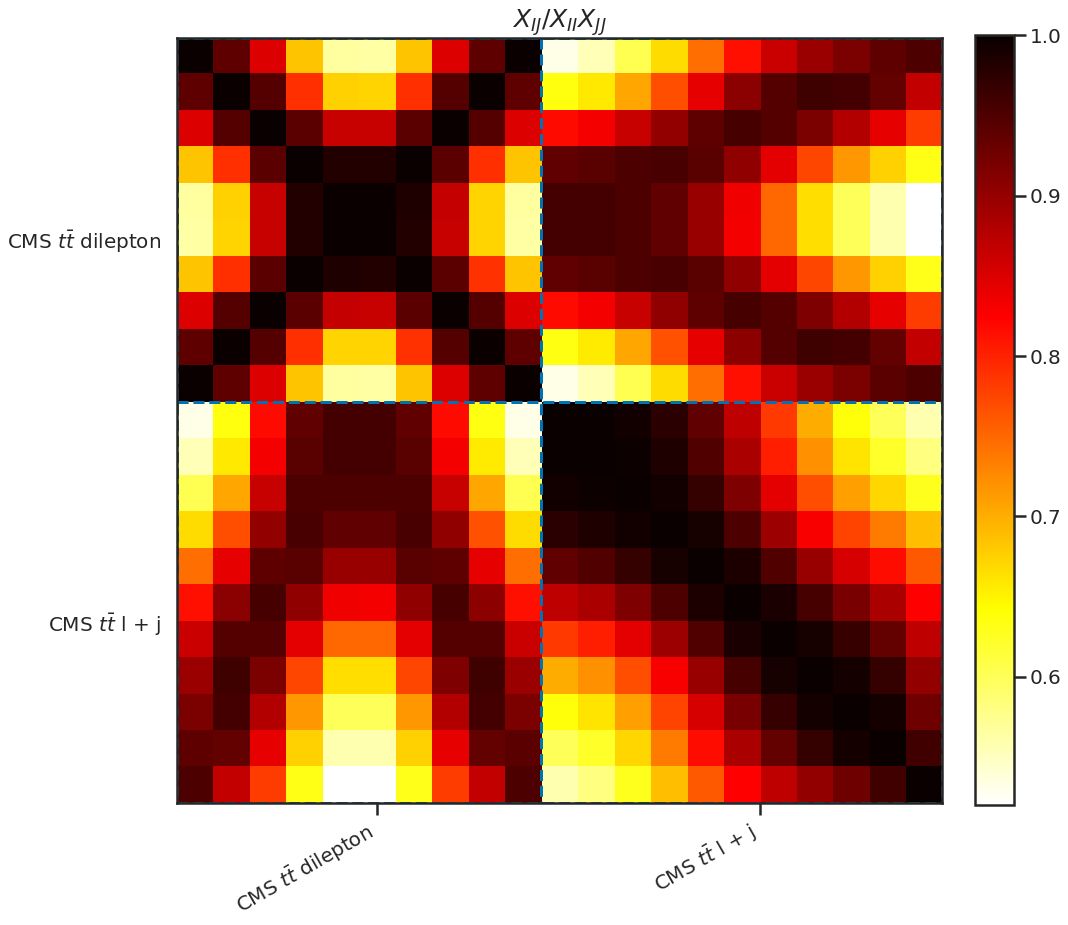
\includegraphics[width=0.48\columnwidth, trim={1.5cm 0 0 0}]{correlations/plots/Xheattop.png}}
   \makebox{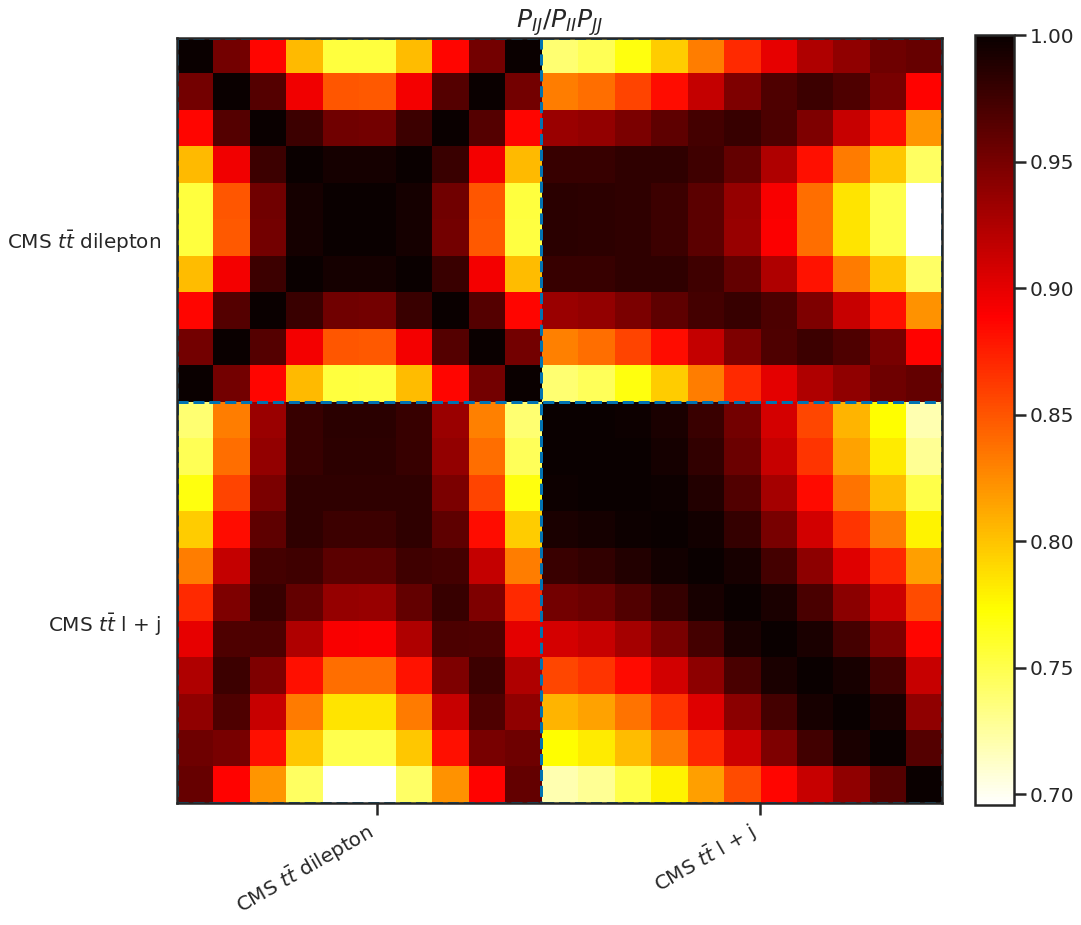
\includegraphics[width=0.48\columnwidth, trim={1.5cm 0 0 0}]{correlations/plots/Pheattop.png}}
    \end{center}
  \vspace{-0.55cm}
  \caption{The left hand plot shows the correlation matrix $\Xtil_{IJ}/\sqrt{\Xtil_{II}\Xtil_{JJ}}$ of the contribution of the PDF uncertainties to the predictions for the 13~TeV rapidity distributions by CMS: the right hand plot shows the correlation matrix $\Ptil_{IJ}/\sqrt{\Ptil_{II}\Ptil_{JJ}}$ of the total uncertainties including the correlated theoretical uncertainties. Note the expanded scales on the heat maps, different in each plot.} 
  \label{fig:CMSttbarcorrlns}
\end{figure}

The theory uncertainties in the predictions are all highly correlated with one another, including between the two rapidity distributions. We can see this by looking at the correlation matrices for $\Xtil$ and $\Ptil$, shown in 
Fig.~\ref{fig:CMSttbarcorrlns}. The predictions are all to start with more than 50\% correlated by the PDF. Then, when correlated theory uncertainties are included, the correlations bump up to $>$ 70\%. We saw before that this is due to the constraint that they must all sum to give the total cross section. The pattern of correlations nicely shows the symmetry within the dilepton distribution, and with the lepton + jets distribution; the greater the rapidity separation, the smaller the correlation.

\subsection{Predicting a new process: Higgs production}
\label{subsec:higgs}
At last we can make some predictions for a new process: one outwith the fit. For this we choose Higgs production via gluon fusion. We calculate the total cross section at 14 TeV using {\tt  ggHiggs}~\cite{Ball:2013bra,Bonvini:2014jma,Bonvini:2016frm}.
Renormalization and factorization scales are set to half the Higgs' mass, and the computation is performed using rescaled effective theory.

\begin{figure}[h]
    \begin{center}
    \makebox{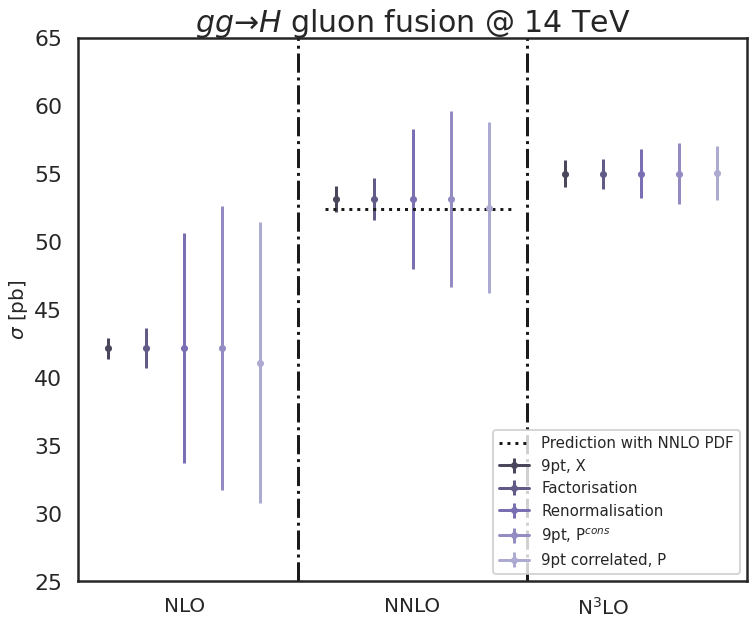
\includegraphics[width=0.6\columnwidth]{correlations/plots/higgs.png}}
    \end{center}
  \vspace{-0.55cm}
  \caption{Predictions for the Higgs total cross-section at 14 TeV, made using a variety of approximations. All results use NLO PDFs, while the Higgs total cross-section is computed at NLO (left panel), NNLO (centre panel) and N$^3$LO (right panel). In each panel, we then have, from left to right: MHOU included only in the PDF determination in the 9pt scheme; the same but with the factorization scale uncertainty (MHOU in PDF evolution) included in quadrature; the same but with instead the renormalization scale uncertainty (MHOU in the Higgs cross-section); the total PDF uncertainty and 9pt MHOU combined in quadrature, as recommended in ~\cite{AbdulKhalek:2019ihb}; the total PDF plus 9pt MHOU, but now including also the shift and the correlation between theoretical uncertainties. In the centre panel we also show the NNLO prediction with NNLO PDFs (but no theoretical uncertainties), as a dashed line. }
  \label{fig:Higgs}
\end{figure}

Our results are shown in in Fig.~\ref{fig:Higgs}. All results use the baseline NLO PDFs with MHOUs, but the parton-level Higgs cross sections are computed at NLO, NNLO and N$^3$LO. We break down the uncertainties into: 
\begin{enumerate}
\item The PDF uncertainty, $\Xtil$;
\item 3-point factorisation scale uncertainty; 
\item 3-point renormalisation scale uncertainty;
\item Uncorrelated (conservative prescription), $\Ptil_{cons}$;
\item Correlated, $\Ptil$.
\end{enumerate}
Note that 2. and 3. sum to give the 5-point prescription in Chapter \ref{chapter:mhous}. 

At NLO the MHOU in the Higgs cross section (estimated by varying the Higgs renormalisation scale) completely dominates the other uncertainties, so the effect of correlations between the sources of MHOU is negligible.  At higher orders, the renormalisation scale uncertainty shrinks dramatically until it is comparable to the other sources of uncertainty at N$^3$LO. Notice also that the shift due to correlations is always very small compared to the overall uncertainty, and gets smaller order by order. Here, unlike for top production, the fit includes no information on Higgs production, so the renormalisation scale is totally uncorrelated. This means any information from the fit must propagate through factorisation scale uncertainties. We can see that at NNLO the small shift due to this pulls the NNLO prediction very close to the calculation using NNLO PDFs, although this is most likely coincidental. The effect of correlations on the total uncertainties is also not very large, and the difference between the simplified and full calculations is small. 

Note that if we used NNLO (or higher order) PDFs with MHOUs here (we can't - they don't exist!), the MHOU in the PDFs would have been smaller, and therefore the effects due to theory uncertainty correlations would be again smaller.

From these examples of autopredictions, and genuine predictions for top and Higgs, we have seen that the extent of the shift and correlation can vary quite significantly, depending on the type of prediction being made and what information is already contained in the PDFs. The conservative prescription recommended in \cite{AbdulKhalek:2019ihb} is certainly not appropriate in general, as the full inclusion of correlations can be quite substantially reduce uncertainties, as we saw both for the autopredictions and top predictions. However, when predicting a new process for which the PDF contains little information about correlated theoretical uncertainties, unsurprisingly the impact of correlations is small and the conservative prescription is sufficient.

\newpage
\section{Summary}
\label{sec:p5}

{\bf \underline{Main conclusion:} When using PDFs which include MHOUs to make predictions, taking account of the correlations between the MHOUs in the PDF and in the predictions can provide significant improvements in accuracy and precision.}

We considered the scenario where PDFs with theory uncertainties are used to make predictions with theory uncertainties. We studied the correlations between these two sources of theory uncertainties. We did this by recasting the theory uncertainties as nuisance parameters for each PDF replica, which contain information about the experimental data's impact on the theory uncertainties. We built our way through increasingly complex and correspondingly realistic models of the fitting procedure, isolating three distinct but related effects, each of which has a significant impact on the final theoretical predictions.

\begin{enumerate}
\item {\bf Shifts in central values: } We understand that we can use experimental data to determine PDFs. But we can also use them to find corrections to the theory which improve the agreement between data and theory. This is done via Bayesian learning through exposure of the fit theory to experimental data. The correlation between the theory uncertainty in the fit and in the predictions then propagates this knowledge through, leading to more accurate predictions. We identified this effect first in Sec.~\ref{sec:p2}.
\item {\bf Learning of theory uncertainties: } In the same mechanism as 1., information from the data is learnt by the fit theory and propagated via correlations to the predictions leading to a reduction in uncertainties. This was also first identified in Sec.~\ref{sec:p2}.
\item {\bf Correlations in theory uncertainties: }The correlations between the theory uncertainties in the fit and those in the prediction lead to a change in the PDF uncertainties in the prediction, even where there isn't a shift. If these correlations are unaccounted for, the theory uncertainty is ``double counted". This was first noted in \cite{Harland-Lang:2018bxd}. The effect is separate to Bayesian learning.
\end{enumerate}

These three effects were found throughout in the simple models in Secs.~\ref{sec:p1}, the one parameter fits in Sec.~\ref{sec:p2} and the multiparameter fits in Sec.~\ref{sec:p3}. Using the NNPDF3.1 NLO global fit with MHOUs, we saw explicitly in Sec.~\ref{sec:p4} that the shifts give reasonable estimates of NNLO corrections, and correspondingly reduce the $\chi^2$ to the experimental data. We also showed that the uncertainty in the NLO predictions can still be thought of as a sum in quadrature of a theory uncertainty and a PDF uncertainty (which itself includes a theory uncertainty). However, these uncertiainties are reduced by a factor that depends on the relative size of the theory and experimental uncertainties, leading to significant shrinking in some cases. The upshot of this is that the conservative prescription is genuinely conservative, sometimes dramatically so. We expect these conclusions to also be true for global fits with fixed parametrisations and tolerance~\cite{Bailey:2020ooq,Hou:2019efy}, were MHOUs to be included. 

We found that the degree of correlation is highly dependent on the type of prediction being made. For the autopredictions (predictions for new measurements of the same data points as those included in the fit), Sec.~\ref{subsec:autopredictions} where there is maximal correspondence between the data in the fit and the predictions being made, the correlation is very high, leading to shifts that improve the quality of the fit to the data, together with a significant reduction in uncertainties, in some cases down to a small fraction of the uncorrelated values. For genuine predictions for new measurements of processes already included in the PDF fit, such as the new measurements of differential top production discussed in Sec.~\ref{subsec:topnhiggs}, we observe that the shift takes the correlated NLO predictions very close to the NNLO prediction, with a significant reduction in uncertainties: the prediction is both more accurate and more precise. For Higgs production, discussed in Sec.~\ref{subsec:higgs}, a process not included in the PDF  fit, the level of correlation is much smaller, since the dominant uncertainty (the MHOU in the hard cross-section) is uncorrelated with the MHOU of the fitted processes. In this case the shift is well within uncertainties, and the reduction in uncertainty very modest, so here the use of the conservative prescription \cite{AbdulKhalek:2019ihb} is entirely appropriate. We expect this to be true of predictions for any new process with large theoretical uncertainties.

The main conclusion is that when using PDFs which include MHOUs to make predictions, taking account of the correlations between the MHOUs in the PDF and in the predictions can provide significant improvements in accuracy and precision. This is especially true if the predicted process is among those included in the fit. 

However, we need to treat the correlated predictions with some care because their reliability is contingent on the appropriate prior being chosen for MHOUs. If too many unjustified assumptions are made, we could end up with predictions that are too aggressive. Bearing this in mind, the conservative (uncorrelated) prescription could have its uses as an upper bound, especially for new processes where we expect the degree of correlation to be low.

In order to calculate fully correlated predictions and uncertainties, one requires besides the PDF replicas some additional  information: the cross-correlations between the theoretical uncertainties in the prediction and those in the theoretical calculations used to determine the PDFs,  $\Shat_{Ij}$; and the cross-correlations between the PDF uncertainties in the prediction and all the calculations included in the fit, $\Xhat_{Ij}$.  In the future, it may be possible to present this information in separate NNPDF deliverables to facilitate the calculation of the correlation effects.

Although we presented our numerical study of correlations in the context of MHOUs, we would expect similar results for other kinds of theoretical uncertainty, such as nuclear uncertainties, higher twist uncertainties, or indeed parametric uncertainties: once the theory covariance matrix has been computed, the linear algebra has no concern for the type of theoretical uncertainty it contains. This suggests a new technique for determining external parameters in PDF fits, such as quark masses or electroweak parameters, taking full account of all correlations with the PDFs and MHOU. We hope to explore this possibility in the near future.
